\section{Introducing an agent}

\newthought{We want to} study the structure of the representations of an agent that can interact with a world.
But before we can study the structure of an agent's representations, we need to define what an agent and its representations are in our framework.

\draftnote{blue}{Include}{
Mention that we use a mix of papers for inspiration for how we define an agent in our framework: Agent as a Markov blanker paper, Higgins, Caselles-Dupre.
OR mention what causes the inspiration as a footnote as we go
}

%%%%%%%%%%%%%%%%%%%%%%%%%%%%%%%%%%%%%%%%%%%%%%%%%%%%%%%%%
\subsection{What is an agent ?}

\newthought{An \emph{agent} is} an autonomous entity\footnote{
    This could be a natural or artificial entity.
} that can observe and interact with a world\footnote{
    Our agent does not need to be embodied in the world - more on this later !
}; the agents that we care about can also learn about the worlds they interact with.

%%%%%%%%%%%%%%%%%%%%%%%%%%%%%%%%%%%%%%%%%%%%%%%%%%%%%%%%%
\subsection{An agent's representation}

\newthought{An agent's \emph{representation states}} are the agent's internal representations of world states, through which the agent maintains its understanding of its world.
An agent's \emph{representation} of the world is the agent's internal model of the world, which includes how the agent encodes and organises information about its world (e.g., as vectors, symbols, or other data structures) as representation states as well as the dynamics of how those representation states change due to actions that affect the world\footnote{
    The agent's representation does not directly encode the dynamics of the world states, it encodes the dynamics of the representation states; a `good' representation will provide a good approximation to the dynamics of the world states.
}.
The agent's representation not only captures the current state of the world but also allows the agent to conceptualise future world states by predicting the world state that will our from the current world state when an action is applied; this allows the agent to plan future actions, and so form a comprehensive framework for decision-making and interaction.

Mathematically, in our framework, we define the agent's representation of the world in the same way as we defined the world: as a multidigraph.
An agent's representation
\begin{equation}
    \mathscr{Z} = (Z, D_{Z}, s_{Z}, t_{Z})
\end{equation}
is a multidigraph consisting of a set $Z$ of representation states, a set $D_{Z}$ of transformations between representation states, a source map $s_{Z}: D_{Z} \to Z$, and a target map $t_{Z}: D_{Z} \to Z$.
All the properties we derived for $\mathscr{W}$ also hold for $\mathscr{Z}$ with the relevant analogue such as the atomic multigraph of the representation
\begin{equation}
    \hat{\mathscr{Z}} = (Z, \hat{D}_{Z}, \hat{s}_{Z}, \hat{t}_{Z}).
\end{equation}

\begin{postulate}
    The most abstract mathematical representation of an agent's representation is a multidigraph that consists of a collection $Z$ of representation states as vertices, a collection $D_{Z}$ of transformations as arrows, a source map $s_{Z}$ that maps each arrow to the world state it is leaving, and a target map $t_{Z}$ that maps each arrow to the world state it is entering.
\end{postulate}

\newthought{Agents use \emph{sensors}} to capture data from their world, enabling the agent to perceive the world; these sensors include real-world sensors (e.g., cameras on a robot, the human eye) and virtual inputs (e.g., data streams, user commands).
Sensors provide the agent with \emph{observation states}\footnote{In some literature, observation states are called \emph{sensory states} such as in \cite{Ramstead2020}.}, which are the agent's internal representations of the information the sensors collect (e.g., data streams from the camera)\footnote{
	Importantly, observation states are not the sensors themselves.
}.
An agent's \emph{perceptual model} is how the agent encodes and organises information from its sensors (e.g., vectors, symbols, or other data structures) as well as how it conceptualises the structure of the landscape of possible observation states.

\newthought{Agents use \emph{effectors}} to interact with and alter worlds.
Effectors enable agents to carry out actions in the world; effectors can be real-world effectors (e.g., motors and actuators on a robot) or virtual outputs (e.g., API calls or applying a transformation to a dataset the agent is manipulating).
Effectors receive \emph{effector signals}\footnote{
Effector signals are commonly called \emph{control signals} in the field of robotics.
}, which are the concrete instructions sent by the agent to perform actions (e.g., a voltage spike sent to a motor or a command sent to a software interface).
An agent also has an \emph{action model}, which is how the agent encodes and organises information about its actions (e.g., control signals, symbolic commands) as well as how it conceptualises how its actions will affect the world state.
An agent's action model is intrinsically linked to its representation since the action model describes the movement between representation states of the representation due to actions\footnote{
These actions do not have to be only the actions of the agent itself, they can be a grouping of world state transformations that the agent understands to be from a particular cause (see \draftnote{blue}{section ???}{}).
}.

%%%%%%%%%%%%%%%%%%%%%%%%%%%%%%%%%%%%%%%%%%%%%%%%%%%%%%%%%
\subsection{Agents as Markov blankets}

\newthought{In our framework}, we consider agents to be systems with internal states that interact with the world such that a boundary is maintained between their internal states and the world.
Agent's in our framework have four types of state:
\begin{enumerate}
	\item \emph{Observation states} represent the agent's inputs from the world (e.g., vision, sound, touch etc...).
	\item \emph{Effector states} represent how the agent influences the world state.
	\item \emph{(External) world states} consist of the states of the agent's external environment, which are the world states we introduced in \cref{sec:A mathematical treatment of worlds and their transformations}.
	\item \emph{Agent's (internal) representation states} contain our agent's representations of the world, memory model, knowledge models, goals, decision making processes etc...
	      These internal states can only interact with the external world states via observation states and effector states.
\end{enumerate}

Using these four types of states, we can view agents in our framework as consisting of internal representation states separated from the external world states by a \emph{Markov blanket} (see \cref{fig:markov_blanket})\footnote{
As we will see, this means that the internal representation states of the agent depend only on the agent's observation states and effector states.
}.

\begin{figure}[H]
	\centering
	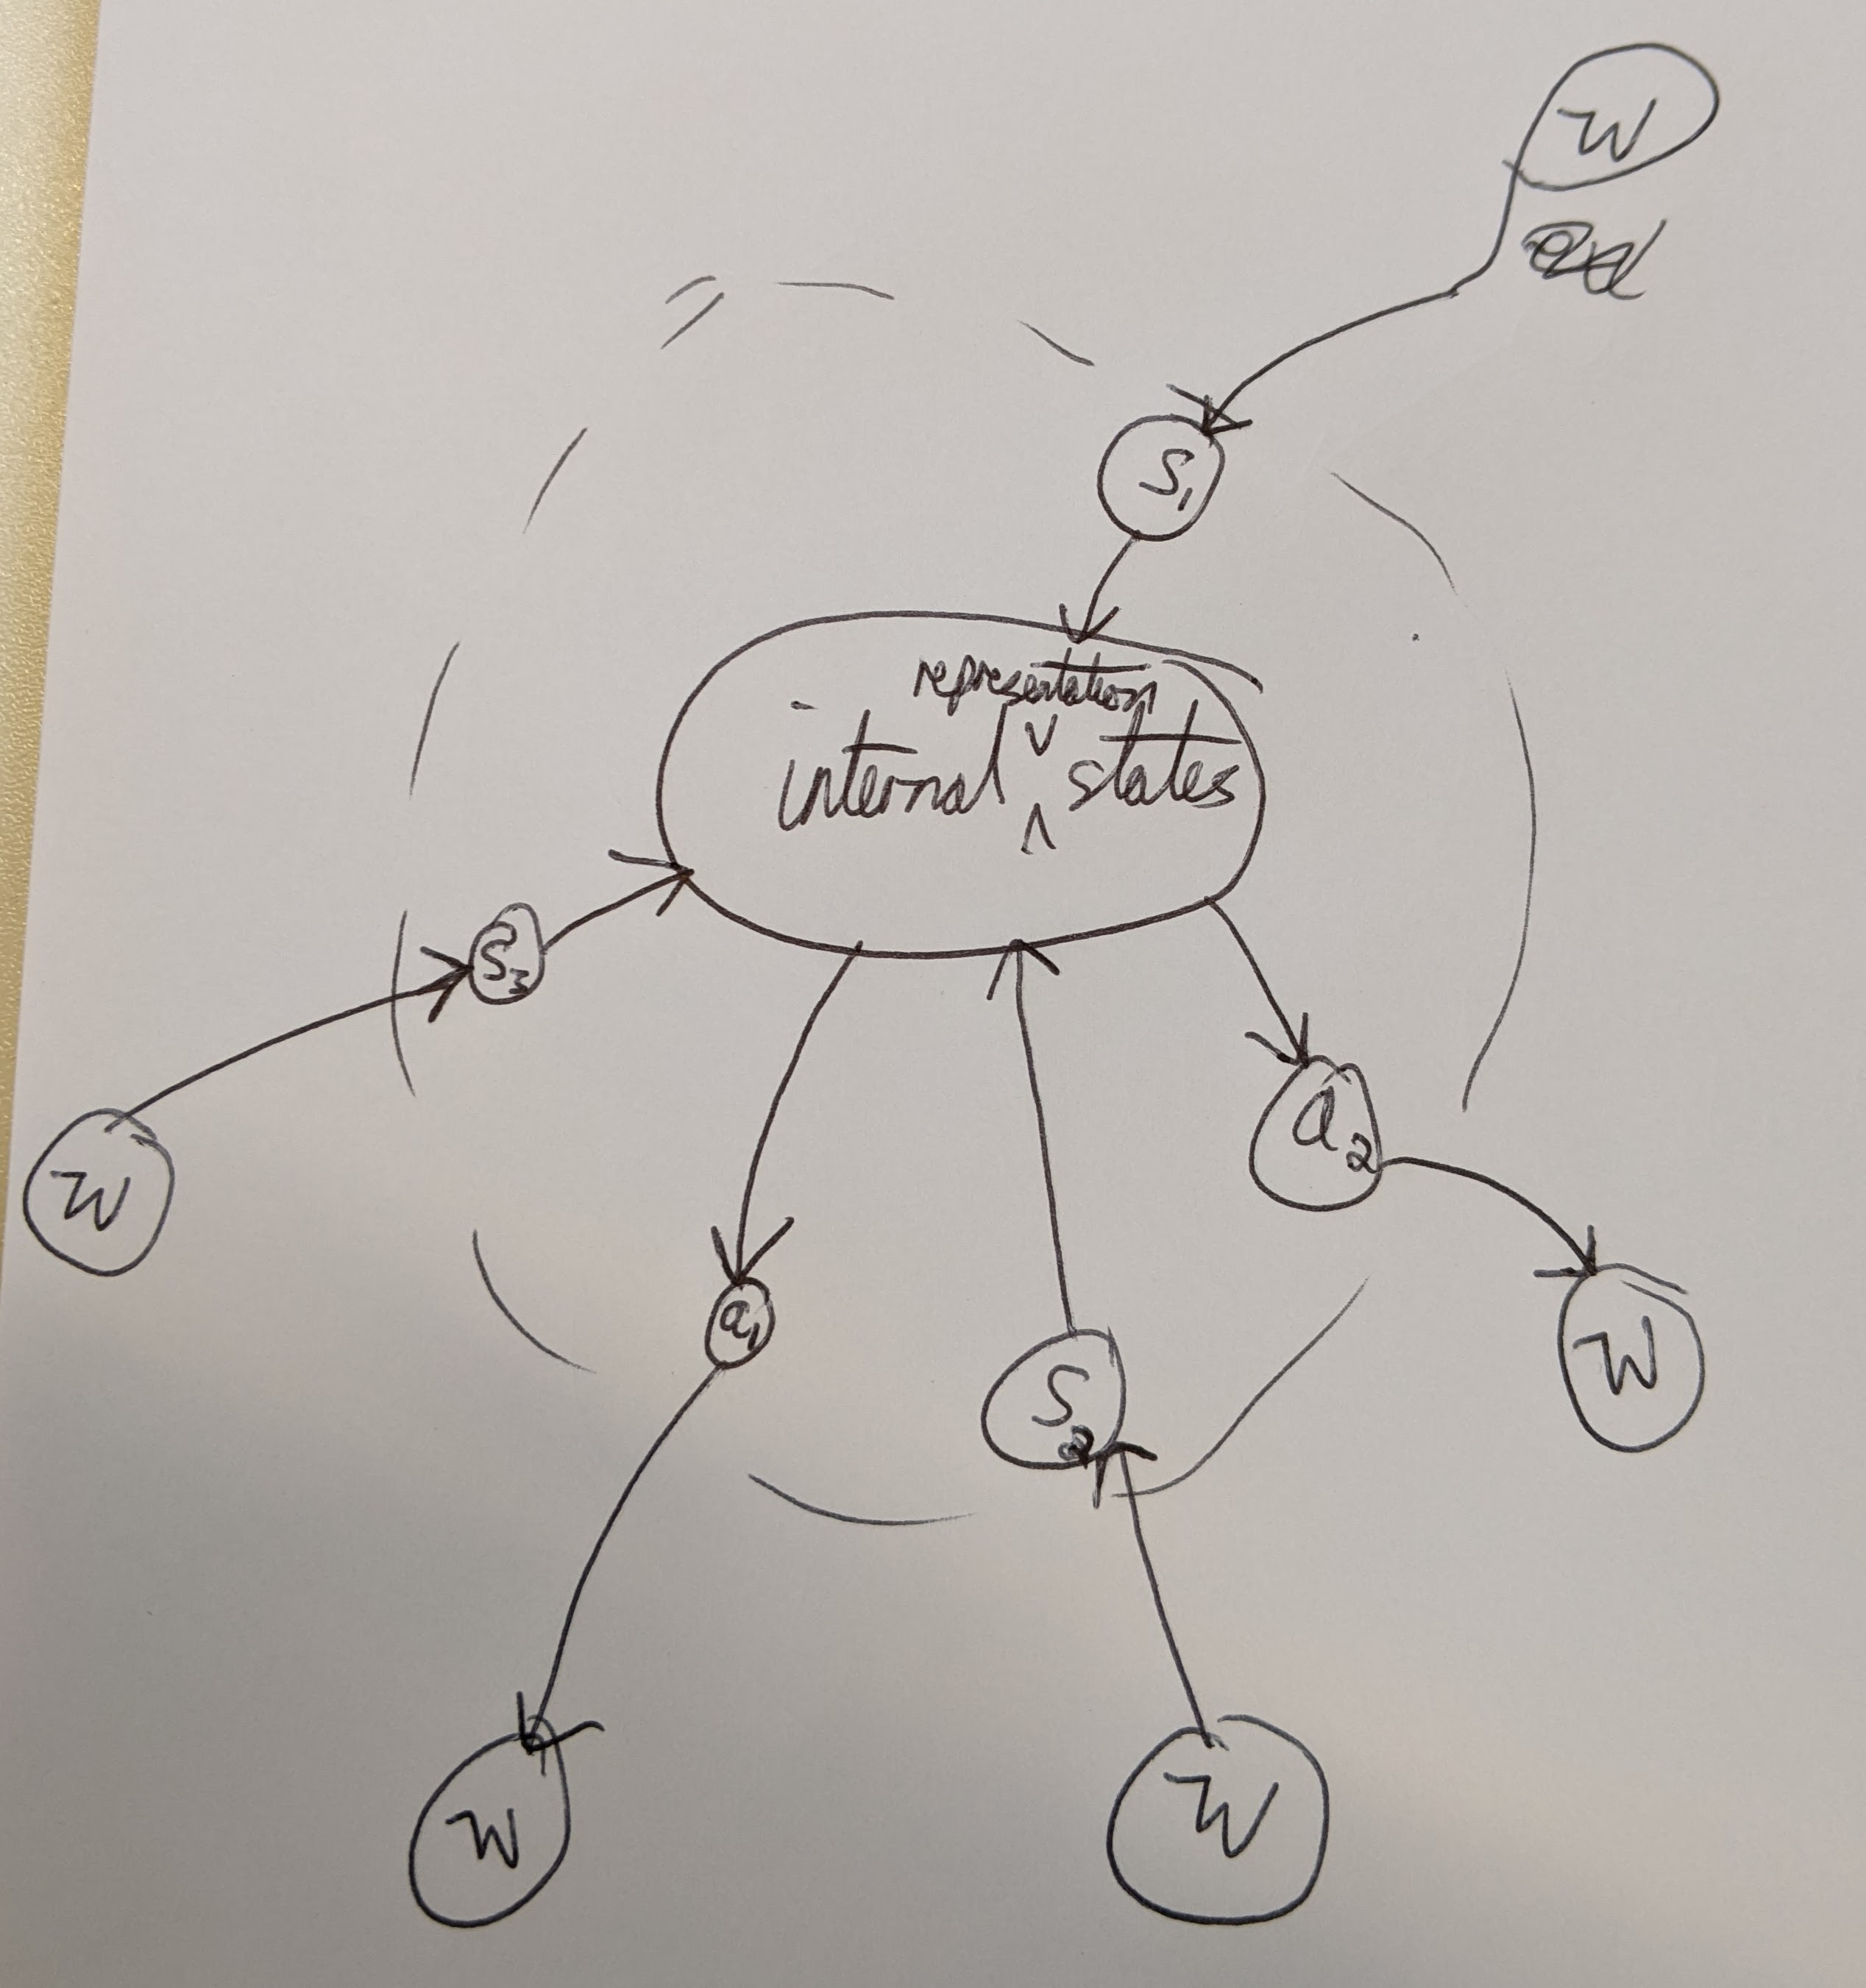
\includegraphics[width=0.5\linewidth]{2MathematicalFramework/Images/markov_blanket.jpg}
	\caption{
		\draftnote{blue}{To do}{Caption}
		Arrows show the flow of information.
        \draftnote{blue}{Agent as a Markov blanket image}{
        % \url{https://www.researchgate.net/figure/The-structure-of-a-Markov-blanket-A-Markov-blanket-highlights-open-systems-exchanging_fig1_343643283}
        }
	}
	\label{fig:markov_blanket}
\end{figure}

The Markov blanket consists of the states that mediate interactions between our agent and its world (i.e., the agent's external environment) \cite{Ramstead2020}.

\newthought{For an agent} in our framework, the observation and effector states form the Markov blanket with the world states being outside the blanket and the the internal state being inside the blanket.
This Markov blanket acts as a boundary that separates the agent's internal representation states from the external world states.
The agent can not directly access the world states, but it can infer the structure of these world states by processing sensory inputs through its observation states and performing actions through its effector states; information about the world states crosses the Markov blanket through the agent's sensory states and the agent's affect on the world crosses the Markov blanket through the agent's effector states.

\begin{postulate}
	An agent consists of internal representation states separated from external world states by a Markov blanket consisting of observation states, through which the agent receives information about the world states, and effectors, through which the agent can change the world state.
\end{postulate}

Technically, given the observation and effector states (i.e., the blanket), the internal representation states of the agent are \emph{conditionally independent} of the external world states; conditionally independent of the external world states means that the behaviour of the agent's internal representation depends only on the states of the agent's Markov blanket (i.e., the agent's observation and effector states) and not (directly) on the world states external to the agent because all the relevant information about the external world states are filtered through the observation states and the agent only affects the world through its effector states.

\newthought{By framing agents} as a Markov blankets, we aim to clearly show that agents learn about their world only through their observation states and their effectors.

A major implication of this approach for our framework is we consider the internal representation states of the agent to be separate from the world states introduced in \cref{sec:A mathematical treatment of worlds and their transformations}; this means that if we swap an agent embodied in a world with another agent that is identical except for having a different internal representation state (or a different representation), then the world state would remain unchanged.

Another implication of our approach is that, since an agent's only gains knowledge about the structure of the world through its sensors and its actions, world states with differences that are not detectable by the agent are identical from the agent's perspective and so can be treated as such when we are constructing a mathematical description of the agent's interaction with the world (i.e, indistinguishable world states do not exist from the perspective of the agent, and so cannot appear in the agent's representation).


%%%%%%%%%%%%%%%%%%%%%%%%%%%%%%%%%%%%%%%%%%%%%%%%%%%%%%%%%
\subsection{Sensory perception}

\newthought{Our agent has} an unspecified number of sensors that allows it to make observations of the world.
Information about the agent's current world state is delivered to the agent's internal decision systems as an observation state; this is called the \emph{observation process}\footnote{
If the world state is modelled as a distribution then is process is also referred to as the agent \emph{sampling the world state}.
}.
For example, the human eye (the sensor) converts information about the light entering the eye into electrical signals in the optic nerve (the observation process); each particular collection of electrical signals (the observation state) is provided to the agent's internal decision mechanisms.

\newthought{Mathematically, we treat} the observation process as a mapping
\begin{equation}
\begin{aligned}
	& b: W \to O \\
	& \text{such that } b(w_{i}) = o_{i}
\end{aligned}
\end{equation}
where $w_{i} \in W$ is a world state and $o_{i} \in O$ the observation state produced by the observation process $b$.
The structure of $o_{i}$ depends on the agent's perceptual model; commonly, each observation $o_{i}$ is a vector of length $N$, where $N$ is the number of sensors the agent has.

\begin{figure}[H]
	\centering
	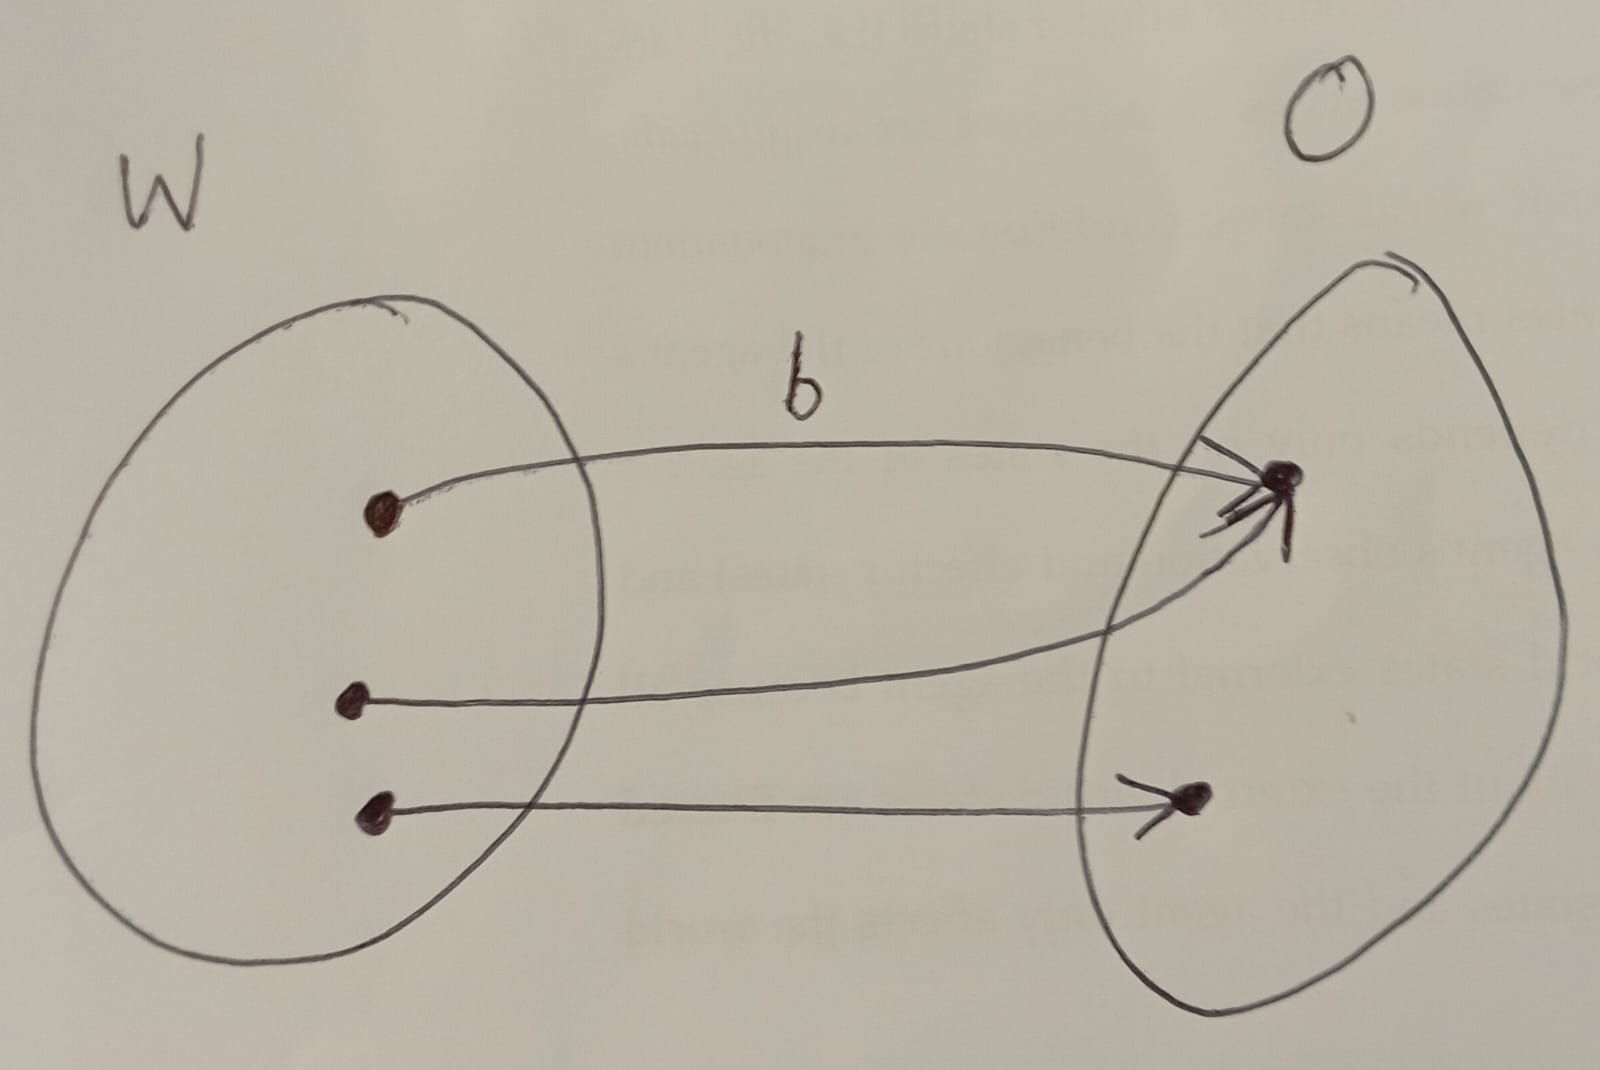
\includegraphics[width=0.5\linewidth]{2MathematicalFramework/Images/observation_process_W_to_O.jpeg}
	\caption{
		An example of how an observation process $b: W \to O$ sends each worlds state in $W$ to an observation state in $O$.
		Note how it is possible for two distinct world states to produce the same observation state.
	}
	\label{fig:observation_process_W_to_O}
\end{figure}


%%%%%%%%%%%%%%%%%%%%%%%%%%%%%%%%%%%%%%%%%%%%%%%%%%%%%%%%%
\paragraph{Ideal sensors.}

\newthought{In real-world situations}, it is common for information about the world state to be lost, modified or not picked up during the observation process (e.g., the human eye only picks up certain wavelengths of light or a camera could capture an image in a colour spectrum then output greyscale) or for distinct world states to produce the same observation state (e.g., worlds where objects can be hidden).
We say that an agent has \emph{ideal sensors}, if
\begin{enumerate}
	\item information is not lost or modified during the observation process;
	\item there is no noise in the obervation process; and
	\item for every distinct world state in $W$ the observation process produces a distinct observation states in $O$:
	\begin{equation}
		b(w) \neq b(w') \quad \text{for all $w,w' \in W$}.
	\end{equation}
\end{enumerate}

Unless stated otherwise, we will only consider agents with ideal sensors\footnote{
Agents with non-ideal sensor are discussed in \draftnote{blue}{section ???}{}
}.


%%%%%%%%%%%%%%%%%%%%%%%%%%%%%%%%%%%%%%%%%%%%%%%%%%%%%%%%%
\paragraph{Partially observable vs fully observable worlds.}

\newthought{If an agent} has complete access to all relevant information about the current world state at any given time\footnote{
This does not mean knowledge of the transformations between world states.
Also, it does not mean knowledge of every world state, but knowledge of the current world state, no matter which world state is the current one
}, then the world is called \emph{fully observable} from the perspective of the agent; if not then the world is called \emph{partially observable} from the perspective of the agent.

\newthought{Partially observable worlds} are common in many real-world scenarios, however, we will initially consider fully observable worlds because
\begin{itemize}
    \item their treatment is mathematically more simple than partially observable worlds because the agent does not have to infer obscured information about world states; and
    \item the representation of an agent of a partially observable world should ideally be the same at the end of the learning process as the representation of the agent in the same world but fully observable\footnote{
    A simple way to turn a fully observable world into a partially observable world would be to add noise to the agent's ideal sensors.
    }; therefore, if we identify structures present in an agent's representation of fully observable worlds then we are also identifying structures that should be present in the agent's representation of the same world but partially observable at the end of the learning process without having to consider the complications of partial observability.
\end{itemize}

%%%%%%%%%%%%%%%%%%%%%%%%%%%%%%%%%%%%%%%%%%%%%%%%%%%%%%%%%
\subsection{Learning and inference}

\newthought{We're interested in} agents that learn about their world.
The end goal of the agent’s learning process is to map the useful aspects of the structure of the world to the structure of its representation\footnote{
The useful aspects are those that enable the agent to complete whatever task the agent has; of course, what is considered to be `useful' depends on the agent's task.
}.
The observation states from our agents' sensors are used by an \emph{inference process} to produce a representation of the current state of the world; the agent then uses some internal mechanism to select an action to perform.
For example, the electrical signals from the optic nerve are given to the brain for inference; mechanisms in the brain then select an action to be performed.

\newthought{Mathematically, we consider} this inference/learning process to be a mapping
\begin{equation}
\begin{aligned}
	& h: O \to Z \\
	& \text{such that } h(o_{i}) = z_{i}
\end{aligned}
\end{equation}
where $o_{i} \in O$ is an observation state and $z_{i} \in Z$ is the representation state the agent associates with the observation state.

\begin{figure}[H]
	\centering
	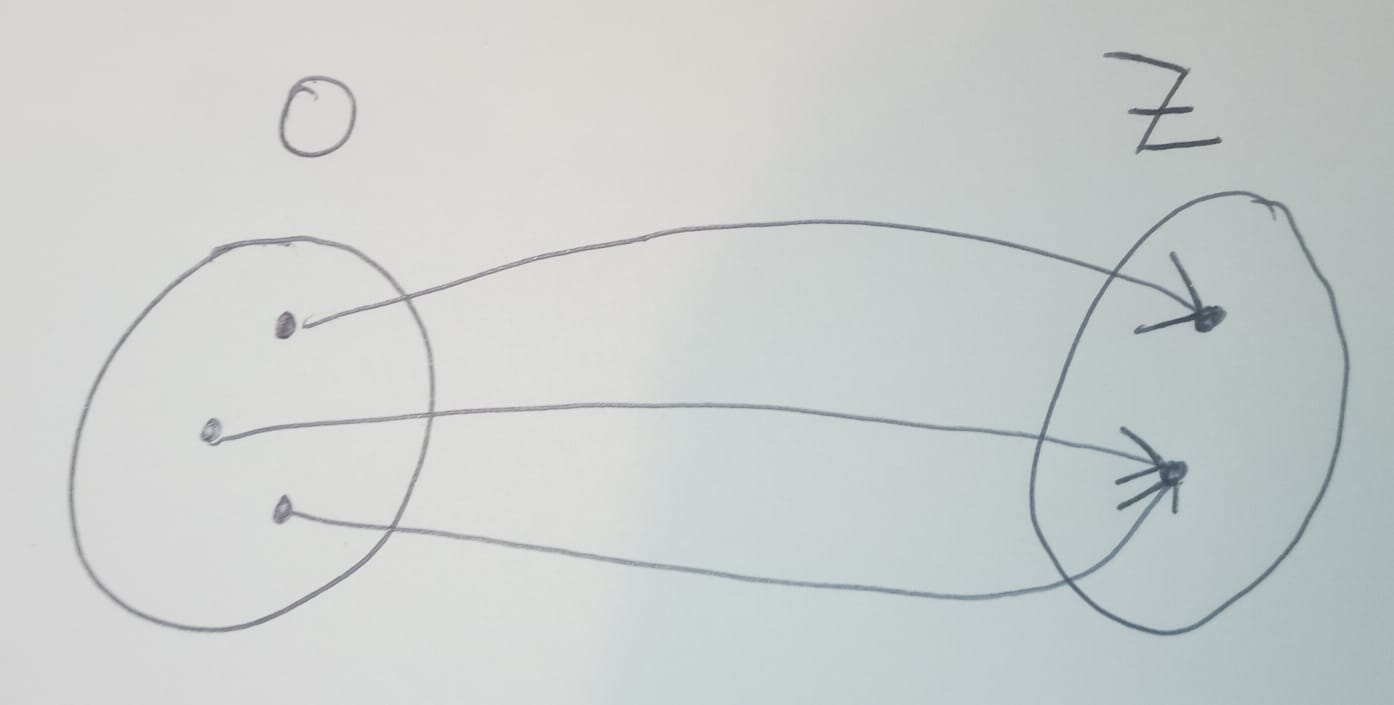
\includegraphics[width=0.5\linewidth]{2MathematicalFramework/Images/inference_process_O_to_Z.jpeg}
	\caption{
		An example of how an inference process $h: O \to Z$ sends each observation state in $O$ to a representation state in $Z$.
		Note how it is possible for two distinct observation states to produce the same representation state.
	}
	\label{fig:inference_process_O_to_Z}
\end{figure}

\newthought{We can combine} $b$ and $h$ to form a mapping
\begin{equation}
\begin{aligned}
	& f: W \to Z \\
	& \text{such that } f = h \circ b
\end{aligned}
\end{equation}
that describes the process of the agent obtaining and processing information about the world.

\begin{figure}[H]
	\centering
	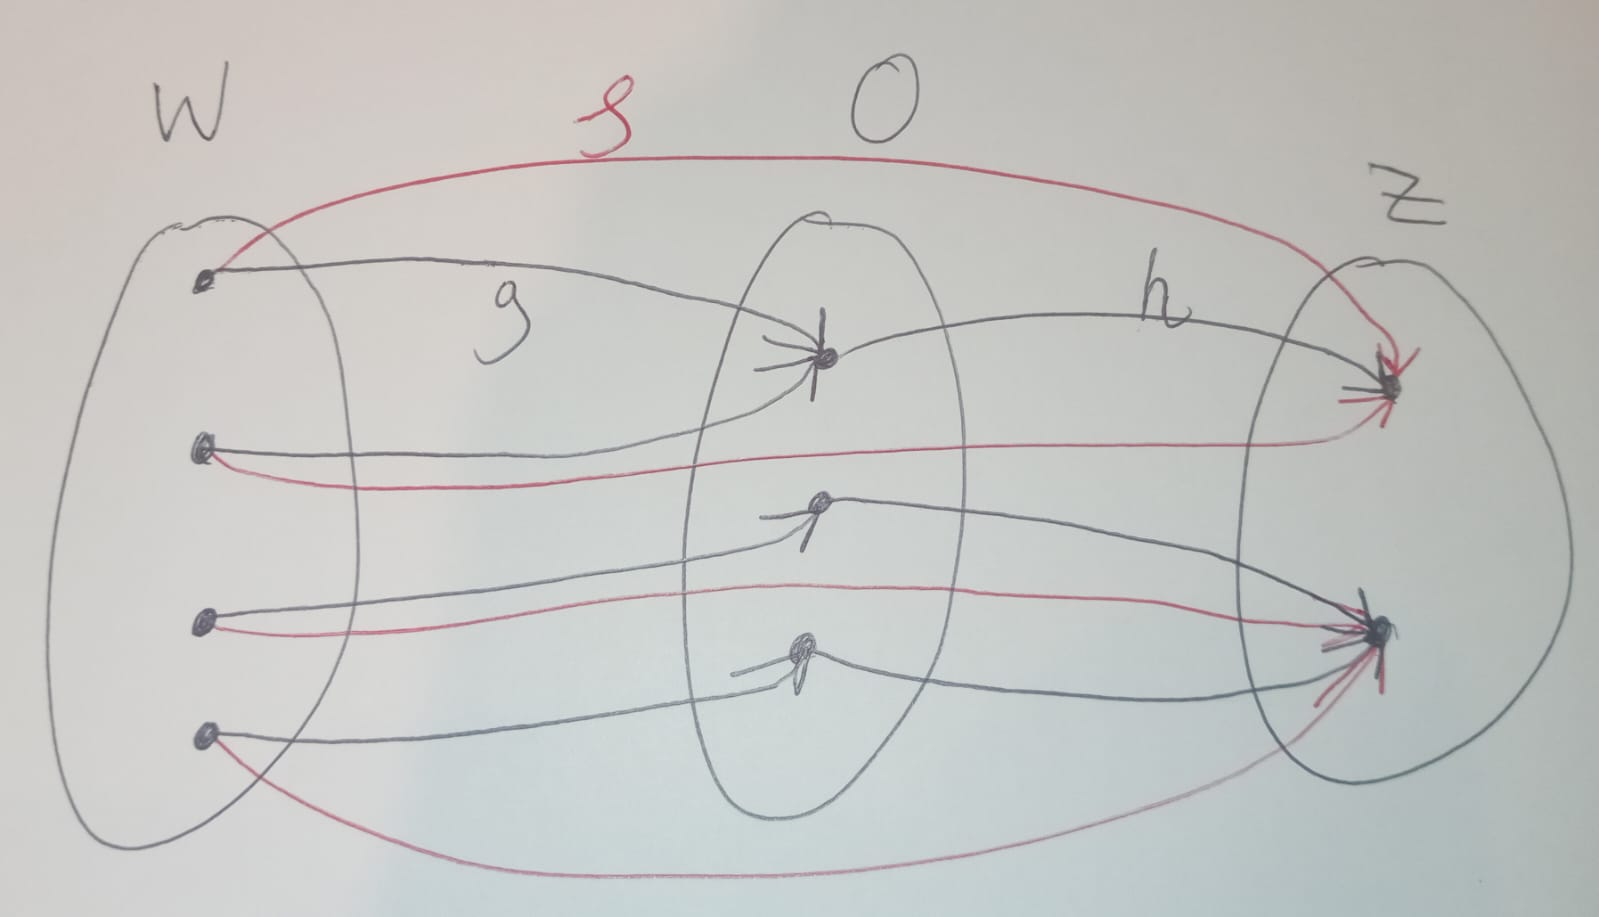
\includegraphics[width=0.5\linewidth]{2MathematicalFramework/Images/W_to_Z.jpeg}
	\caption{
		An example of the map $f: W \to Z$ sends each world state in $W$ to a representation state in $Z$.
		\draftnote{blue}{awjdean}{$g$ should be $b$.}
	}
	\label{fig:W_to_Z}
\end{figure}


\begin{propositionE}[][normal]
    For agents with ideal sensors \draftnote{blue}{consider}{and a perfect learning process}, the map $f$ is bijective.
\end{propositionE}
\begin{proofE}
	\draftnote{blue}{awjdean}{Proof that $f$ is bijective if agent ideal sensors.
	1. Prove $b$ bijective.
	2. Prove $h$ bijective.
	3. Composition of two bijective maps is also a bijective map.
}
\end{proofE}

\draftnote{purple}{PS}{
Figure showing $W$ to $O$ to $Z$ mappings for an agent with \textbf{ideal sensors}.
}

%%%%%%%%%%%%%%%%%%%%%%%%%%%%%%%%%%%%%%%%%%%%%%
\subsection{Our approach to studying an agent's learning}
\draftnote{blue}{Consider}{Move this up ?}

\newthought{We initially focus} on studying the structure of the worlds $\mathscr{W}$ directly, rather than the structure of agent's representations $\mathscr{Z}$.
This is useful because
\begin{enumerate}
    \item since both a world and an agent's representation of the world are general multidigraphs, any propositions we derive on the world are also true for agent's representations\footnote{
    Note that this does not mean that specific properties of a world $\mathscr{W}$ are always found in the representation $\mathscr{Z}$ of an agent interacting with that world, just that the general properties of worlds are also the general properties of representations.
    };
    
    \item we assume that a `good' learning algorithm should produce representations of a world that reflect the relevant structure of the world in the structure of the agent's representation\footnote{
    In other words, a `good' learning algorithm produces agent's representation $\mathscr{Z}$ that are homomorphic to aspects of the world $\mathscr{W}$.
    \draftnote{blue}{Consider}{
    Homomorphic vs isomorphic to a subworld of the world $\mathscr{W}$
    }
    }, so if we identify these relevant structures in the world we know what we want the end result of our agent's learning to be\footnote{
    Essentially we can treat the multidigraph of the world as the ground truth of the agent's representation at the end of the learning process.
    }, potentially aiding the design of learning algorithms that produce those structures;

    \item since we are concerned with the structure of the agent's representation at the end of the learning process our results are agnostic to any learning algorithm which has a path independent learning process (i.e., learning algorithms where the order that information is received by the algorithm doesn't change the end result of the learning); and

    \item if we prove that worlds that do not obey certain conditions cannot have certain properties, then the representation produced by a good learning algorithm will not have those properties irrespective of the details of the learning algorithm.
\end{enumerate}

%%%%%%%%%%%%%%%%%%%%%%%%%%%%%%%%%%%%%%%%%%%%%%%%%%%%%%%%%%%%%%%%%%%
\subsection{An agent, mathematically}

In our framework, an agent
\begin{equation}
    \mathscr{A} = (\hat{A}, \mathscr{Z}, b, h)
\end{equation}
consists of a set $\hat{A}$ of atomic actions\footnote{
Note that we're continuing to use a $\hat{}$ to denote something is atomic, contains atomic things, or that an operator acts exclusively on atomic things.
}, a representation $\mathscr{Z}$, an observation process $b$, and an inference process $h$.

%%%%%%%%%%%%%%%%%%%%%%%%%%%%%%%%%%%%%%%%%%%%%%%%%%%%%%%%%%%%%%%%%%%
\section{Actions of agents}

\draftnote{blue}{To do}{Improve this intro.}
\newthought{In this section}, we define the actions of agents as collections of transformations that are labelled by their associated action.
We then define some relevant properties of these actions.

%%%%%%%%%%%%%%%%%%%%%%%%%%%%%%%%%%%%%%%%%%%%%%%%%%%%%%%%%%%%%%%%%%%
\subsection{Actions as collections of labelled transformations}

\newthought{Consider an agent} $\mathscr{A}$ with a set $\hat{A}$ of atomic actions that can interact with a world $\mathscr{W} = (W, D)$.
We now take the Kleene star operator of $\hat{A}$ \footnote{
	$\hat{A}^{*} = \{ \varepsilon \} \cup \{ (\hat{a}_1, \hat{a}_2, \dots, \hat{a}_n) \mid \hat{a}_i \in \hat{A}, \, n \in \mathbb{N} \}$.
} to get the set of all possible finite sequences formed from elements of $\hat{A}$, including the empty sequence, which we call the \emph{empty action} and denote by $\varepsilon$.
We call $\hat{A}^{*}$ the set of \emph{actions of the agent}, and we call the elements of $\hat{A}^{*}$ \emph{actions}\footnote{
Sometimes we refer to the elements of $\hat{A}^{*}$ as \emph{sequences of actions}.
}.

\newthought{We define a} composition operator
\begin{equation}
	\circ: \hat{A}^{*} \times \hat{A}^{*} \to \hat{A}^{*}
\end{equation}
such that $(a_1, a_2, \dots, a_n) \in \hat{A}^{*}$ can be written as $a_1 \circ a_2 \circ \dots \circ a_n$.
The operator $\circ$ is the concatenation of strings.

\begin{corollaryE}
    $\circ$ is closed by the definition of the Kleene star operator and the concatenation of strings.
\end{corollaryE}

\begin{corollaryE}\label{col:circ_associative}
    $\circ$ is associative by definition of the Kleene star operator and the concatenation of strings.
\end{corollaryE}

\begin{notation}
	Sometimes we write compositions like $a_1 \circ a_2 \circ \dots \circ a_n$ as $a_1 a_2 \dots a_n$.
\end{notation}


Each action $a \in \hat{A}^{*}$ is either the empty action ($a = \varepsilon$) or $a$ can be expressed as unique sequences of composed atomic actions\footnote{
This follows from the definition of the Kleene star operator.
}:
\begin{equation}
    \operatorname{Seq} : \left\{ 
    \begin{array}{l}
        \hat{A}^{*} \backslash \{\varepsilon\} \to \hat{A}^{n} \\
        \{\varepsilon\} \to \{\varepsilon\}
    \end{array} \right.
\end{equation}
such that
\begin{align}
    & \operatorname{Seq}(a) = (\hat{a}_{n}, \hat{a}_{n-1}, \dots, \hat{a}_{1}) \quad \text{for $a = \hat{a}_{n} \circ \hat{a}_{n-1} \circ \dots \circ \hat{a}_{1}$} \\
    & \operatorname{Seq}(\varepsilon) = \varepsilon.
\end{align}


\paragraph{Length of an action.}
\newthought{The \emph{length} $|a|$ of} an action $a \in \hat{A}^{*}$ is the number of atomic actions in the action's the unique sequence of atomic actions\footnote{
	This means atomic actions have a length of one.
}.


\paragraph{The empty action $\varepsilon$.}
\newthought{The empty action} $\varepsilon$ has the following properties:
\begin{enumerate}
    \item \textbf{Uniqueness.}
    There is only one empty action $\varepsilon$.
    \item \textbf{Identity element for concatenation.}
    The empty action $\varepsilon$ serves as an identity element for concatenation of sequences:
    \begin{align}
        \label{eqn:empty_action_is_left_identity}
        & \varepsilon \circ a = a \quad \text{for all $a \in \hat{A}^{*}$} \\
        \label{eqn:empty_action_is_right_identity}
        & a \circ \varepsilon = a \quad \text{for all $a \in \hat{A}^{*}$}
    \end{align}
    \item \textbf{Length.}
    The empty action $\varepsilon$ has a length of zero
    \begin{equation}
        |\varepsilon| = 0.
    \end{equation}
\end{enumerate}

%%%%%%%%%%%%%%%%%%%%%%%%%%%%%%%%%%%%%%%%%%%%%%%%%%%%%%%%%%%%%%%%%%%
\paragraph{Linking actions with transformations.}

\newthought{We now want} to link the elements of our set $\hat{A}^{*}$ of actions to the transformations in $D$ which would occur if an agent performed each action while in each world state.
We do this by first labelling transformations in the set $D$ of transformations that are caused by atomic actions in $\hat{A}$, then by labelling the compositions of those transformations with the relevant actions in $\hat{A}^{*}$ taking into account which compositions of atomic actions form each of the actions in $\hat{A}^{*}$.

\begin{postulate}
	Actions are collections of labelled transformations.
\end{postulate}

\newthought{Let $\hat{D}_{A} \subset D$ be the} set of transformations that are caused by the atomic actions in $\hat{A}$; we call $\hat{D}_{A}$ the set of \emph{atomic action transformations}.
We define a labelling map
\begin{equation}
    \hat{l}: \hat{D}_{A} \to \hat{A}
\end{equation}
such that any two distinct atomic transformations leaving the same world state are labelled with different actions:
\begin{equation}
  \text{If } s(d) = s(d'), \text{ then } \hat{l}(d) \neq \hat{l}(d') \quad \text{for any } d, d' \in \hat{D}_{A}.
\end{equation}
We call $\hat{l}$ the \emph{atomic action labelling map}.

Now, we will use $\hat{D}_{A}$ to construct a multidigraph with arrows that are labelled by the atomic action labelling map $l$.
Let $\hat{\mathscr{W}}_{\mathscr{A}}$ be the subworld of $\mathscr{W}$\footnote{
    Note that in general $\hat{\mathscr{W}}_{\mathscr{A}} \centernot\subseteq \hat{\mathscr{W}}$ because the transformation caused by an atomic action does not need to be an atomic transformation.
}
\begin{equation}
    \hat{\mathscr{W}}_{\mathscr{A}} \subseteq \mathscr{W}
\end{equation}
such that
\begin{equation}
    \hat{\mathscr{W}}_{\mathscr{A}} = (W, \hat{D}_{A})
\end{equation}
We now use the atomic action labelling map to label the arrows in $\hat{\mathscr{W}}_{\mathscr{A}}$ and give a labelled multidigraph which we also denote by $\hat{\mathscr{W}}_{\mathscr{A}}$.
We call $\hat{\mathscr{W}}_{\mathscr{A}}$ the \emph{atomic multidigraph of the actions of the agent}.

\newthought{We can now} apply the same method of taking the set of all finite directed walks we used previously when constructing $\mathscr{W}$ from $\hat{\mathscr{W}}$ to our atomic multidigraph $\hat{\mathscr{W}}_{\mathscr{A}}$ to give
\begin{equation}
    \mathscr{W}_{\mathscr{A}} = (W, D_{A});
\end{equation}
We call $\mathscr{W}_{\mathscr{A}}$ the \emph{world restricted to the actions of the agent $\mathscr{A}$}, and we call the set $D_{A}$ the set of \emph{transformations due to the actions of the agent $\mathscr{A}$}.

We can naturally extend the atomic action labelling map $\hat{l}$ to a map $l$, called the \emph{action labelling map}\footnote{
    The construction of $l$ from the agent's perspective happens during the learning process.
}, as
\begin{equation}
    l: D_{A} \to \hat{A}^{*}
\end{equation}
such that $l$ satisfies the following conditions:
\begin{enumerate}
    \item Any two distinct transformations leaving the same world state are labelled with different actions:\footnote{
    This could be viewed as a condition of the world being deterministic.
    }
    \begin{actioncondition}[Uniqueness]\label{actcon:action_gives_single_outcome}
      For any $d,d' \in D_{A}$ with $s(d)=s(d')$, $l(d) \neq l(d')$.
    \end{actioncondition}

    \item Trivial transformations, $1_{w}$ for all $w \in W$, are mapped to the empty action $\varepsilon$:
    \begin{actioncondition}[Identity]\label{actcon:trivial_transformations_mapped_to_empty_sequence}
      $l(1_{w}) = \varepsilon$ for all $w \in W$.
    \end{actioncondition}

    \item Transformations are labelled consistently with the sequence of labels corresponding to their constituent atomic transformations.
    \begin{actioncondition}[Composition consistency]\label{actcon:composition_consistency}
      If $d = \hat{d}_{n} \circ ... \circ \hat{d}_{1}$ then $l(d) = \hat{l}(\hat{d}_{n}) ... \hat{l}(\hat{d}_{1})$ for all $d \in D_{A}$ and for all $\hat{d_{1}}, \dots , \hat{d_{n}} \in \hat{D}_{A}$.
    \end{actioncondition}
\end{enumerate}
Using the action labelling map $l$, $\mathscr{W}_{\mathscr{A}}$ becomes a labelled multidigraph.

\whendraft{
\draftnote{purple}{Note}{This is currently under whendraft.}
A summary of the procedure we have taken to label the transformations of a world $\mathscr{W}$ that are due to the actions of an agent is given by \cref{fig:action_labelling_procedure}.

\begin{figure}[H]
	\centering
	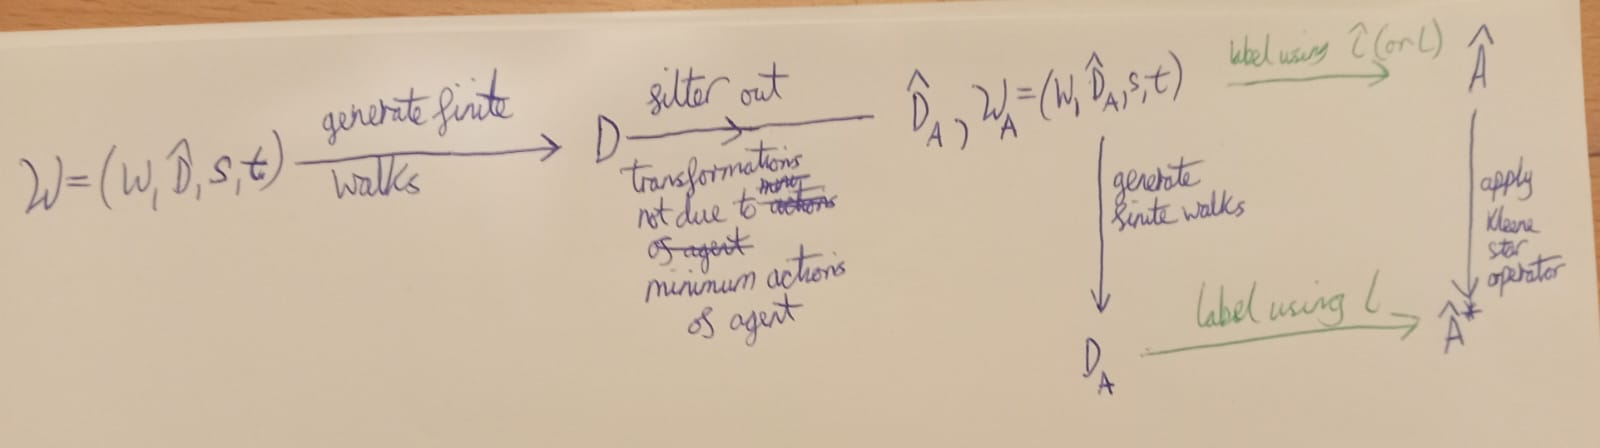
\includegraphics[width=\linewidth]{2MathematicalFramework/Images/action_labelling_procedure.jpeg}
	\caption{
    Procedure for labelling the transformations of the world with their associated action.
    \draftnote{blue}{To do}{This might need updating.}
    }
	\label{fig:action_labelling_procedure}
\end{figure}
\draftnote{purple}{End of whendraft}{}
}

\begin{notation}
    For a transformation $d \in D_{A}$ with $d: w \to w'$ and $l(d) = a$, we will often denote $d$ by $d: w \xrightarrow{a} w'$.
\end{notation}

\newthought{It is clear,} that the construction of $\mathscr{W}_{\mathscr{A}}$ requires both the world $\mathscr{W}$ and the agent $\mathscr{A}$; therefore it makes sense to consider world-agent pairs $\mathscr{W}$-$\mathscr{A}$ instead of worlds and agents individually\footnote{
We provide an empirical proof of how changing the set of atomic actions of an agent can alter the algebraic structure of the agent's representation in \draftnote{blue}{section ???}{}.
}.
\draftnote{purple}{PS}{Reword this.}

\newthought{For the rest} of this thesis we only consider worlds $\mathscr{W}$ where all the transformations of the world are due to the actions of an agent $\mathscr{A}$; in other words, worlds $\mathscr{W}$ where
\begin{equation}
    \hat{\mathscr{W}} = \hat{\mathscr{W}}_{\mathscr{A}}.
\end{equation}
We also assume the learning process is \emph{perfect}; at the end of a perfect learning process, the agent's representation $\mathscr{Z}$ exactly matches the structure of the world $\mathscr{W}_{\mathscr{A}}$.


\paragraph{Effect of actions on world states.}
\newthought{Unlike transformations, which} are fixed by their source and target world states, actions can have different outcomes when applied to different world states.
For example, it could be the case that applying the action $a$ followed by the action $b$ on a world state $w_{1}$ gives back the original world state, while applying $a$ followed by $b$ on world state $w_{2}$ could give a different world state $w_{3}$\footnote{
This differing behaviour is due to how the action $a$ labels particular transformations in $D$
}.
Due to this behaviour, we need a way to describe how actions change world states.

\newthought{We define the} \emph{action effect operator} $\ast$, which gives the effect of an action $a \in \hat{A}^{*}$ on a world state $w \in W$, as
\begin{equation}
	\ast: \hat{A}^{*} \times W \to W
\end{equation}
such that
\begin{enumerate}
	\item if there exists a $d: w \xrightarrow{a} t(d)$, then $a \ast w = t(d)$; and
	\item if there does not exist a $d: w \xrightarrow{a} t(d)$, then we say that $a \ast w$ is \emph{undefined}.
\end{enumerate}


\begin{propositionE}
    $\ast$ is well-defined.
\end{propositionE}
\begin{proofE}
    Suppose there exist two transformations $d, d' \in D_{A}$ with $d: s(d) \xrightarrow{a} t(d)$ and $d': s(d) \xrightarrow{a} t(d')$ for some $a \in \hat{A}^{*}$.
    From \cref{actcon:action_gives_single_outcome},
    \begin{equation}
        s(d)=s(d') \text{ and } l(d)=l(d') \implies d = d'.
    \end{equation}
    It follows that
    \begin{equation}
         d = d' \implies t(d) = t(d').
    \end{equation}
    Therefore, if the effect $a \ast w$ is defined, then the target state $t(d)$ is unique.
\end{proofE}


\begin{propositionE}
    \label{prp:circ_ast_compatibility}
    $\ast$ and $\circ$ are compatible:
    \begin{equation}\label{}
        (a' \circ a) \ast w = a' \ast (a \ast w) \quad \text{for any $a, a' \in \hat{A}^{*}$ and $w \in W$}
    \end{equation}
\end{propositionE}
\begin{proofE}
    \draftnote{purple}{PS}{Improve this.}
    This follows naturally from the composition consistency property on the labelling map $l$.
    If $d_{1}: w \xrightarrow{a} w'$ and $d_{2}: w' \xrightarrow{a'} w''$, then $d_{2} \circ d_{1}: w \xrightarrow{a' \circ a} w''$.
    By the definition of $\ast$, $a * w = t(d_{1})$, $a' \ast (a \ast w) = t(d_{2})$, and $(a' \circ a) \ast w = t(d_{2} \circ d_{1})$.
    Therefore, since $d_{2} \circ d_{1}$ has the label $a' \circ a$, we see that $(a' \circ a) \ast w = a' \ast (a \ast w)$.
\end{proofE}

\Cref{prp:circ_ast_compatibility} means that $\ast$ is an \emph{action} of the algebra $(\hat{A}^{*}, \circ)$ on the set $W$ \footnote{
    The action of an algebra is different to the actions of an agent.
    Yes, it's confusing!
}.
Another consequence of \cref{prp:circ_ast_compatibility} is that we can express any action $a \in \hat{A}^{*}$ as a unique sequence of atomic actions using $\operatorname{Seq}$ and then apply each of these atomic actions one at a time\footnote{
We can also split actions into shorter, but not atomic sequences of actions and apply each of those sequences individually: if $\operatorname{Seq}(a) = (\hat{a}_{k} \dots, \hat{a}_{1})$, then
\begin{align}
	a \ast w & = (\hat{a}_{k} \dots \hat{a}_{3}) \ast (\hat{a}_{2} \ast (\hat{a}_{1} \ast w))  \\
	         & = (\hat{a}_{k} \dots \hat{a}_{3}) \ast ((\hat{a}_{2} \circ \hat{a}_{1}) \ast w) \\
	         & = \dots
\end{align}
}:
if $\operatorname{Seq}(a) = (\hat{a}_{k}, \dots, \hat{a}_{1})$, then
\begin{align}
    a \ast w & = (\hat{a}_{k} \dots \hat{a}_{1}) \ast w                                       \\
     & = (\hat{a}_{k} \dots \hat{a}_{2}) \ast (\hat{a}_{1} \ast w)                    \\
     & = (\hat{a}_{k} \dots \hat{a}_{3}) \ast (\hat{a}_{2} \ast (\hat{a}_{1} \ast w)) \\
     & = \dots
\end{align}

We can restrict the action effect operator $\ast$ to the set of atomic actions $\hat{A}$ to give the \emph{atomic action effect operator}:\footnote{
    $\hat{\ast}$ and $\ast$ describe the interactions between a world and an agent; therefore, $\hat{\ast}$ and $\ast$ are not properties of agents or of worlds, they are properties of world-agent pairs.
}
\begin{equation}
    \hat{\ast}: \hat{A} \times W \to W.
\end{equation}

\begin{propositionE}
    For a world-agent pair $\mathscr{W}$-$\mathscr{A}$, the set $W$ of world states, the set $\hat{A}$ of atomic actions, and the values of the atomic action effect operator $\hat{\ast}$ are sufficient to generate $\mathscr{W}_{\mathscr{A}}$; in other words,
    \begin{equation}
        \mathscr{W}_{\mathscr{A}} := (W, \hat{\ast})
    \end{equation}
\end{propositionE}
\begin{proofE}
    First, we construct the set $\hat{A}^{*}$ by applying the Kleene star operator.
    Then, since we can express any action $a \in \hat{A}^{*}$ as a unique sequence of atomic actions $\operatorname{Seq}(a)$, we have that, for any $w \in W$ and $a \in \hat{A}^{*}$, we can work out $a \ast w$ by applying each of its the atomic in sequence:
    if $\operatorname{Seq}(a) = (a_{n}, a_{n-1}, \dots, a_{1})$,
    \begin{equation}
        a \ast w = a_{n} \hat{\ast} (a_{n-1} \hat{\ast} (\dots \hat{\ast} (a_{1} \hat{\ast} w)\dots))
    \end{equation}
    Then we can construct the associated transformation in $D_{A}$ as $d: w \xrightarrow{a} a \ast w$.
    
    Constructing a transformation in this way for all pairs $(w, a) \in W \times \hat{A}^{*}$ gives us the set $D_{A}$, and therefore we have
    \begin{equation}
        \mathscr{W}_{\mathscr{A}} = (W, D_{A}).
    \end{equation}
\end{proofE}

\draftnote{purple}{PS}{
(figure in margin) Diagram showing what $W$, $Z$, $A$, $w$, $z$, $a$ are.
}

\newthought{At the end} of learning process, if the atomic action effector operator in the agent's representation matches the atomic action effector operator of the world, then the atomic multidigraph $\hat{\mathscr{Z}}$ will be isomorphic to the atomic multidigraph of $\hat{\mathscr{W}}$.

%%%%%%%%%%%%%%%%%%%%%%%%%%%%%%%%%%%%%%%%%%%%%
\subsection{Actions as (partial) functions.}

\newthought{Consider all the} transformations that are labelled by a particular action $a \in \hat{A}^{*}$.
Together these transformations form a partial function $f_{a}: W \to W$ because for any $w \in W$ either $a \ast w$ is undefined or $a \ast w$ is defined and there is a unique world state $w' \in W$ for which $a \ast w = w'$ (from \cref{actcon:action_gives_single_outcome}).
Each of the transformations labelled by the action $a$ is an assignment of $f_{a}$ to one of the world states in $W$ ($f_{a}(w) \mapsto a \ast w = w'$).

Formally, we can curry\footnote{Currying is an operation that allows us to transform an operation with multiple arguments into a collection of functions with single arguments by fixing all but one of the operation's arguments.} the action effect operator $\ast : \hat{A}^{*} \times W \to W$
\begin{equation}
	\operatorname{Curry}: (\ast: \hat{A}^{*} \times W \to W) \to (f_{a}: W \to W)
\end{equation}
to obtain a collection of (partial) functions
\begin{equation}
	\mathcal{T}_{\hat{A}^{*}} = \{f_{a}: W \to W \mid f_{a}(w) = a \ast w \text{ where defined, for each } a \in \hat{A}^{*} \}
\end{equation}

These functions $f_{a}$
\begin{enumerate}
    \item are not generally surjective because for a given $w \in W$ there is not necessarily a transformation $d \in D$ with $l(d) = a$ and $t(d) = w$ \draftnote{purple}{PS}{Illustrative diagram}.

    \item are not generally injective because it is possible to have an world where $f_{a}(w)=f_{a}(w')$ for some $w \in W$ different from $w' \in W$ \draftnote{purple}{PS}{Illustrative diagram}.
\end{enumerate}


%%%%%%%%%%%%%%%%%%%%%%%%%%%%%%%%%%%%%%%
\subsection{Reachable subworlds due to the actions of an agent}

To define the \emph{reachable subworld due to the actions of an agent}, we take the reachable subworld definition and replace $\hat{D}$ with $\hat{D}_{A}$.
For a world-agent pair $\mathscr{W}$-$\mathscr{A}$,
\begin{align}
	 & W^{\mathscr{A}\to}(w) := \{ w' \in W \mid \text{there exists} \; d \in D_{A} \; \text{with} \; d: w \to w' \} \\
	 & \hat{D}_{A}^{\mathscr{A}\to}(w) := \{ \hat{d} \in \hat{D}_{A} \mid s(\hat{d}) \in W^{\mathscr{A}\to}(w) \; \text{and} \; t(\hat{d}) \in W^{\mathscr{A}\to}(w) \} \\
	 & \hat{\mathscr{W}}^{\mathscr{A}\to}(w) := (W^{\mathscr{A}\to}(w), \hat{D}_{A}^{\mathscr{A}\to}(w), \hat{s} \big|_{\hat{D}_{A}^{\mathscr{A}\to}(w)}, \hat{t} \big|_{\hat{D}_{A}^{\mathscr{A}\to}(w)})
\end{align}
where $W^{\mathscr{A}\to}(w)$ is the set of world states that are reachable from the world state $w \in W$ using the actions of the agent, $\hat{D}_{A}^{\mathscr{A}\to}(w)$ is the set of atomic transformations that are reachable from $w$ using the actions of the agent, and $\hat{\mathscr{W}}^{\mathscr{A}\to}(w)$ is the atomic multigraph of the reachable subworld of $\mathscr{W}$ from $w$ using the actions of the agent $\mathscr{A}$.
The reachable subworld $\mathscr{W}^{\mathscr{A}\to}(w)$ is then constructed from $\hat{\mathscr{W}}^{\mathscr{A}\to}(w)$ in the usual way.
The natural reachable subworld due to the actions of the agent is denoted by $\mathscr{W}^{\mathscr{A}\to}(w^{*})$.


%%%%%%%%%%%%%%%%%%%%%%%%%%%%%%%%%%%%%%%
\subsection{Totalisation: from partial to total}

\newthought{Partial functions can} be difficult to deal with.
However, we can turn our partial functions into total functions (totalisation) while keeping the undefined behaviour of the partial functions by introducing a new world state $\bot$ to our set $W$ of world states, where $\bot$ represents the \emph{undefined world state}\footnote{
    This technique for turning partial functions into total functions is used in functional programming languages like Haskell \cite{marlow2010haskell}.
}.
This gives us an augmented set of world states:
\begin{equation}
	W^{\bot} = W \cup \{ \bot \}
\end{equation}

We also extend the effect $\ast : \hat{A}^{*} \times W \to W$ of actions on world states to $\ast^{\bot} : \hat{A}^{*} \times W^{\bot} \to  W^{\bot}$ so that if $a \ast w$ is defined then it remains the same as before, but if $a \ast w$ is undefined, then we set $a \ast^{\bot} w$ equal to our undefined state $\bot$:\footnote{
    Note that we have:
    \begin{equation}
        a \ast^{\bot} \bot = \bot \quad \text{for all $a \in \hat{A}^{*}$}
    \end{equation}
    which means that $\bot$ acts as an \emph{absorbing element} for $\ast^{\bot}$.
}
\begin{align}
	 & \ast^{\bot} : \hat{A}^{*} \times W^{\bot} \to  W^{\bot} \quad\text{such that} \\
	 & a \ast^{\bot} w =
	\begin{cases}
		a \ast w & \text{if there exists a $d \in D_{A}$ with $d: w \xrightarrow{a} t(d)$}, \\
		\bot & \text{otherwise.}
	\end{cases}
\end{align}
If we say $a \ast w$ is defined we mean $a \ast w \neq \bot$, and if we say that $a \ast w$ is undefined we mean $a \ast w = \bot$ \footnote{
    If, for example, there are multiple failure modes that we want our agent to learn, we can introduce multiple undefined world states $\bot_{1}, \bot_{2}, \bot_{3} \dots$ to allow our agent to keep track of the different "types" of undefined.
}.

\newthought{We can augment} $D_{A}$ so that we have transformations that reflect the behaviour of $\ast^{\bot}$ by including transformations that send world states to $\bot$ if $a \ast^{\bot} w = \bot$.

First, we define the set $\Delta^{\bot}$ of new transformations that terminate at $\bot$, which includes transformations for $a \ast^{\bot} \bot$:
\begin{alignat}{2}
    & U {}={} && \{ (a,w) \in \hat{A}^{*} \times W \mid \not\exists (d: w \xrightarrow{a} t(d)) \in D_{A} \} \\
    & \Delta^{\bot} {}={} && \{ d^{\bot}: w \xrightarrow{a} \bot \mid (a, w) \in U \}                                       \\
                  &       && \cup \{ d^{\bot}: \bot \xrightarrow{a} \bot \text{ for all $a \in \hat{A}^{*}$} \} \\
    & D_{A}^{\bot} = && D \cup \Delta^{\bot}
\end{alignat}

We now extend our action labelling map $l: D_{A} \to \hat{A}^{*}$ to include our new $\bot$-terminating transformations:
\begin{align}
	 & l^{\bot} : D_{A}^{\bot} \to \hat{A}^{*} \quad\text{such that} \\
	 & l^{\bot}(d) =
	\begin{cases}
		l(d) & \text{if $d \in D_{A}$}, \\
		a    & \text{if $d \in \Delta^{\bot}$ and $d: s(d) \xrightarrow{a} \bot$.}
	\end{cases}
\end{align}

\begin{notation}
    To simplify notation, we will use $W$, $\ast$, $D_{A}$, and $l$ to denote $W^{\bot}$, $\ast^{\bot}$, $D_{A}^{\bot}$, and $l^{\bot}$ respectively for the rest of this thesis.
    If we want to explicitly use the non-augmented set of world states (not containing $\bot$), we will use $W^{\centernot\bot}$.
\end{notation}


%%%%%%%%%%%%%%%%%%%%%%%%%%%%%%%%%%%%%%%%%
\section{
Structures\texorpdfstring{: $(\hat{A}^{*}, \circ)$, $\mathcal{T}_{\hat{A}^{*}}$, and $(\hat{A}^{*}, \circ, \ast)$}{}
}

\newthought{In this section}, we will look at three notable algebraic structures: $(\hat{A}^{*}, \circ)$, $\mathcal{T}_{\hat{A}^{*}}$, and $(\hat{A}^{*}, \circ, \ast)$.

\newthought{$(\hat{A}^{*}, \circ)$ is the free} monoid generated by the set $\hat{A}$.
This means there are no relations between the generators in $\hat{A}$ apart from the associativity and identity $\varepsilon$ required for $(\hat{A}^{*}, \circ)$ being a monoid, and so $(\hat{A}^{*}, \circ)$ provides maximum flexibility in constructing elements\footnote{
Note that the structure of $(\hat{A}^{*}, \circ)$ is unaffected by the effect $\ast$ of actions on world states.
}.
$(\hat{A}^{*}, \circ)$ is also decidable: there exists an algorithm that can decide if two elements in $\hat{A}^{*}$ are identical in finite time.


\begin{propositionE}
    $(\hat{A}^{*}, \circ)$ is a monoid.
\end{propositionE}
\begin{proofE}
\begin{enumerate}
    \item \textbf{Total.}
    By definition of the Kleene star operator, an action in $\hat{A}^{*}$ is a finite sequence of atomic actions in $\hat{A}$.
    Since any sequence in $\hat{A}^{*}$ can be expressed as a unique sequence of atomic actions in $\hat{A}$, for any two such finite sequences $a, a' \in \hat{A}^{*}$, their concatenation $a' \circ a$ is also a finite sequence of elements of $\hat{A}$ and so $a' \circ a \in \hat{A}^{*}$.
    
    \item \textbf{Associativity.}
    $\circ$ is associative for all $a \in \hat{A}^{*}$ from \cref{col:circ_associative}.

    \item \textbf{Identity element.}
    The empty action $\varepsilon \in \hat{A}^{*}$ acts as the identity element.
    From \cref{eqn:empty_action_is_left_identity,eqn:empty_action_is_right_identity} we have
    \begin{align}
        & \varepsilon \circ a = a \quad \text{for all $a \in \hat{A}^{*}$} \\
        & a \circ \varepsilon = a \quad \text{for all $a \in \hat{A}^{*}$}
    \end{align}
\end{enumerate}
\end{proofE}


\newthought{The structure $(\hat{A}^{*}, \circ, \ast)$ is} a \emph{monoid action}\footnote{
\whendraft{
\draftnote{blue}{This footnote is under a whendraft}{}
\begin{definition}[Monoid action]
    A monoid action is a monoid $(M, \cdot)$ and a set $X$ together with an action
    \begin{equation}
        \ast: M \times X \to X
    \end{equation}
    satisfying
    \begin{enumerate}
        \item \textbf{Identity.}
        For all $x \in W$,
        \begin{equation}
            e \ast x = x
        \end{equation}
        where $e$ is the identity element of $(M, \cdot)$.
        \item \textbf{Compatibility.}
        For all $m,n \in M$ and for all $x \in X$,
        \begin{equation}
            (m \circ n) \ast x = m \ast (n \ast x)
        \end{equation}
    \end{enumerate}
\end{definition}
}
}.


\begin{propositionE}
	$(\hat{A}^{*}, \circ, \ast)$ is a monoid action of $\hat{A}^{*}$ on the set $W$.
\end{propositionE}
\begin{proofE}
\begin{enumerate}
    \item \textbf{Compatibility.}
          The action effect operator $\ast$ is compatible with the composition operator $\circ$ since:
          \begin{equation}
              (a' \circ a) \ast w = a' \ast (a \ast w) \quad \text{for all $a, a' \in \hat{A}^{*}$ and $w \in W$}.
          \end{equation}

    \item \textbf{Identity.}
          The empty action $\varepsilon$ acts as the identity on $W$:
          \begin{equation}
              \varepsilon \ast w = w \quad \text{for all } w \in W.
          \end{equation}
\end{enumerate}
\end{proofE}

While the structure of the free monoid $(\hat{A}^{*}, \circ)$ does not depend on the world $\mathscr{W}$, the structure of $(\hat{A}^{*}, \circ, \ast)$ does depend on the world $\mathscr{W}$.


\newthought{Now we have} introduced the undefined state $\bot$, the set $\mathcal{T}_{\hat{A}^{*}}$ is a set of (total) functions $f_{a}: W \to W$ with one $f_{a}$ for each action $a \in \hat{A}^{*}$ \footnote{
Making the $\bot$'s explicit, $\mathcal{T}_{\hat{A}^{*}}$ is now defined as:
\begin{equation}
\begin{aligned}
    \mathcal{T}_{\hat{A}^{*}} = \{ & f_{a}: W^{\bot} \to W^{\bot} \mid                                \\
                                      & f_{a}(w) = a \ast^{\bot} w \text{ for $a \in \hat{A}^{*}$} \}
\end{aligned}
\end{equation}
}.
$\mathcal{T}_{\hat{A}^{*}}$ is the \emph{transformation monoid} that results from the monoid action of $\hat{A}^{*}$ on $W$.


\begin{propositionE}
    \label{prp:T_is_monoid}
    $\mathcal{T}_{\hat{A}^{*}}$ is a monoid under composition $\cdot: \mathcal{T}_{\hat{A}^{*}} \times \mathcal{T}_{\hat{A}^{*}} \to \mathcal{T}_{\hat{A}^{*}}$ of functions with:
    \begin{equation}
        f_{a}(w) = a \ast w
    \end{equation}
    for all $a \in \hat{A}^{*}$ and $w \in W$.
\end{propositionE}
\begin{proofE}
\begin{enumerate}
    \item \textbf{Compatibility.}
    For any $w \in W$ and any $a, a' \in \hat{A}^{*}$,
    \begin{align}
        (f_{a'} \cdot f_{a})(w) & = f_{a'} (f_{a}(w)) \\
        & = a' \ast (a \ast w) \\
        & = (a' \circ a) \ast w \\
        & = f_{a' \circ a}(w)
    \end{align}

    \item \textbf{Associativity.}
    Associativity of the composition of the partial functions $f_{a}$ follows from the associativity of $\circ: \hat{A}^{*} \times \hat{A}^{*} \to \hat{A}^{*}$:
    \begin{align}
      (f_{a''} \cdot f_{a'}) \cdot f_{a} & = f_{a'' \circ a'} \cdot f_{a}       \\
                                         & = f_{(a'' \circ a') \circ a}         \\
                                         & = f_{a'' \circ (a' \circ a)}         \\
                                         & = f_{a''} \cdot f_{a' \circ a}       \\
                                         & = f_{a''} \cdot (f_{a'} \cdot f_{a})
    \end{align}
    \item \textbf{Identity element.}
    The function $f_{\varepsilon}$ that corresponds to the empty action $\varepsilon$ is the identity function:
    \begin{equation}
      f_{\varepsilon}(w) = \varepsilon \ast w = w \quad \text{for all $w \in W$}
    \end{equation}

    For any $a \in \hat{A}^{*}$, we have
    \begin{equation}
        f_{a} \cdot f_{\varepsilon} = f_{a \circ \varepsilon} = f_{a}
    \end{equation}
    and
    \begin{equation}
        f_{\varepsilon} \cdot f_{a} = f_{\varepsilon \circ a} = f_{a},
    \end{equation}
    which is the definition of $f_{\varepsilon}$ being the identity.
\end{enumerate}
\end{proofE}

\draftnote{purple}{PS}{
Put monoid homomorphism part into a proposition ?
}
There exists a monoid homomorphism\footnote{
    $\phi$ arises directly due to the \emph{universal property of free monoids}.
    We take a mapping $a \mapsto f_{a}$ that assigns each atomic action $a \in \hat{A}$ to its corresponding effect function $f_{a}$.
    Then, by the universal property of free monoids, $a \mapsto f_{a}$ uniquely extends to a monoid homomorphism $\phi : \hat{A}^{*} \to \mathcal{T}_{\hat{A}^{*}}$ that preserves the monoid structure.

    Another interesting property of the universal property of free monoids is that any monoid homomorphism from $(\hat{A}^{*}, \circ)$ to any monoid $M$, then that homomorphism is uniquely determined by what it does on the generators in $\hat{A}$;
    this is because every element in $\hat{A}^{*}$ can be expressed as a unique sequence of atomic actions.

    Note that $\phi$ is not necessarily \emph{faithful} because it is possible for two distinct actions $a, a' \in \hat{A}^{*}$ to give transformations with the same effect for every world state:
    \begin{equation}
        f_{a}(w) = a \ast w = a' \ast w = f_{a'}(w)
    \end{equation}
    for all $w \in W$.
} from $(\hat{A}^{*}, \circ)$ to $\mathcal{T}_{\hat{A}^{*}}$:
\begin{equation}
    \label{eqn:monoid_homomorphism_from_free_monoid_to_set_of_functions}
    \phi : \hat{A}^{*} \to \mathcal{T}_{\hat{A}^{*}} \quad\text{defined by $\phi(a) = f_{a}$}
\end{equation}
that preserves the monoid structure
\begin{align}
	 & \phi(a' \circ a) = f_{a' \circ a} = f_{a'} \cdot f_{a} = \phi(a') \cdot \phi(a) \\
	 & \phi(\varepsilon) = f_{\varepsilon}
\end{align}

Each function $f_{a}$ precisely represents the effect of an action $a \in \hat{A}^{*}$ on all possible world states.
Other properties of $f_{a} \in \mathcal{T}_{\hat{A}^{*}}$ include:
\begin{enumerate}
    \item \textbf{Not generally invertible.}
    There may not exist a function $f_{a}^{-1}$ such that $f_{a}^{-1} \circ f_{a} = f_{a} \circ f_{a}^{-1} = f_{\varepsilon}$.
    \item \textbf{Not necessarily injective.}
    It is possible for a function $f_{a}$ to map different world states to the same world state (i.e., it is possible to have $f_{a}(w) = f_{a'}(w)$).
    \item \textbf{Not necessarily surjective onto $W$.}
    It is possible for there to be a world state that is not reachable through a function $f_{a}$ (i.e., it is possible for a $w \in W$ to exist such that there is no $w' \in W$ where $f_{a}(w') = w$ for some $a \in \hat{A}^{*}$).
\end{enumerate}

\newthought{Without totalisation from} augmenting $W$ with $\bot$, $(\hat{A}^{*}, \circ)$ is unchanged, $(\hat{A}^{*}, \circ, \ast)$ is the partial action of the monoid $(\hat{A}^{*}, \circ)$ on $W$, and $(\mathcal{T}_{\hat{A}^{*}}, \cdot)$ is the monoid of partial transformations on $W$ that results from the partial monoid action of $\hat{A}^{*}$ on $W$.


%%%%%%%%%%%%%%%%%%%%%%%%%%%%%%%%%%%%%%%%%%%%%%%%%%%%%%%%%%%%%%%%%%%%%%%%%%%%%%%%%%%%%%%%%%%%%%
\section{
An example world \texorpdfstring{$\mathscr{W}_{\alpha}$}{}
 }\label{sec:an_example_world}

\newthought{So far we} have seen a lot of definitions and propositions, now we will illustrate these ideas through a toy example world.
Our chosen toy world is a $2\times 2$ cyclic grid world $\mathscr{W}_{\alpha}$, where all the transformations in $\mathscr{W}_{\alpha}$ are due to the actions of an agent $\mathscr{A}$ embodied in the world\footnote{
This toy world $\mathscr{W}_{\alpha}$ was inspired by the worlds given in \cite{Higgins2018,caselles2019symmetry}.
}.


%%%%%%%%%%%%%%%%%%%%%%%%%%%%%%%%%%%%%%%%%%%%%%%%%%%%%%%%%%%%%%%%%%%%%%%%%%%%%%%%%%%%%%%%%%%%%%
\subsection{
World states of $\mathscr{W}_{\alpha}$
}\label{sec:World states of example}

The world states of $\mathscr{W}_{\alpha}$ are shown in \cref{fig:2x2-cyclical-grid-world-states}:
\begin{equation}
    W = \{ w_{1}, w_{2}, w_{3}, w_{4} \}
\end{equation}

\begin{figure}[H]
	\centering
	\begin{subfigure}[b]{0.45\linewidth}
		\centering
		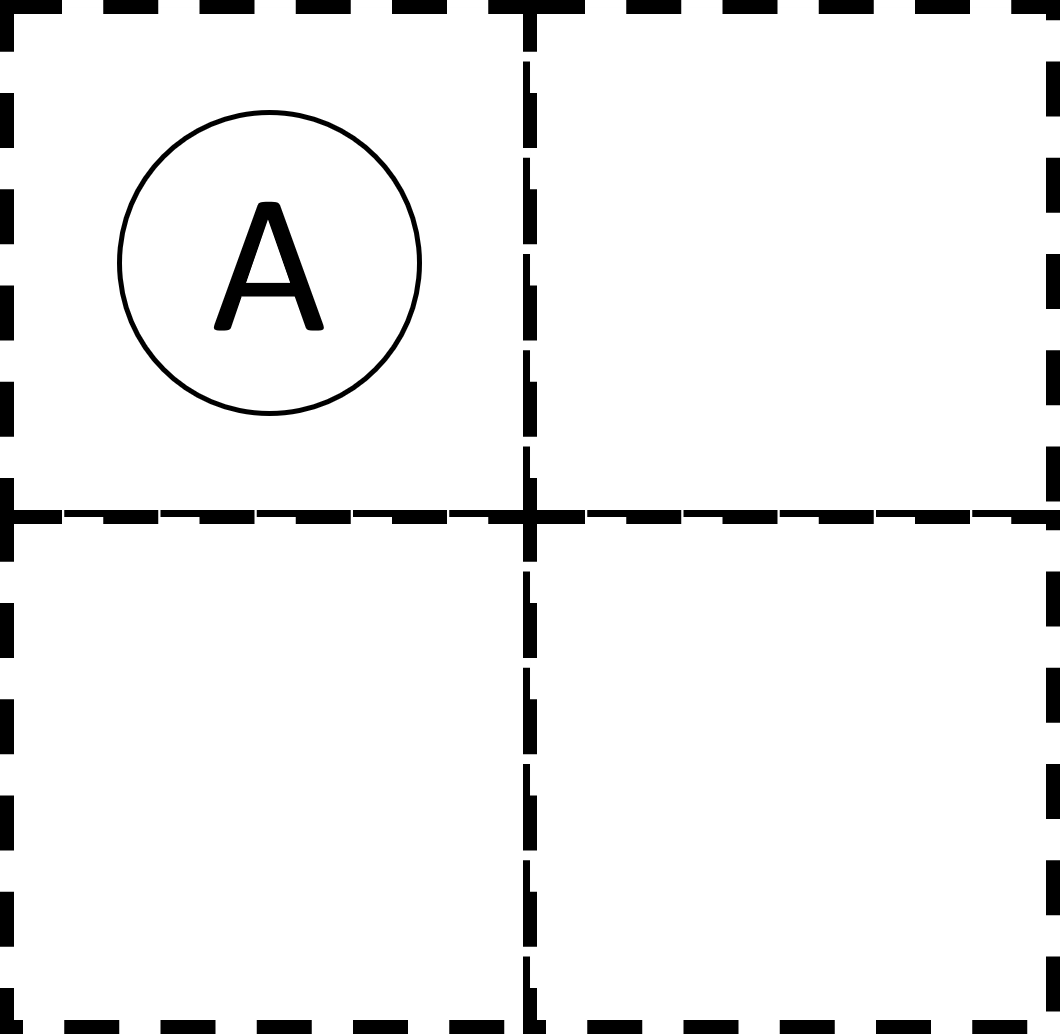
\includegraphics[width=0.5\linewidth]{2MathematicalFramework/Images/2x2_no_walls_world_states/w0.png}
		\caption{$w_{1}$}
		\vspace{0.25cm}
	\end{subfigure}
	\begin{subfigure}[b]{0.45\linewidth}
		\centering
		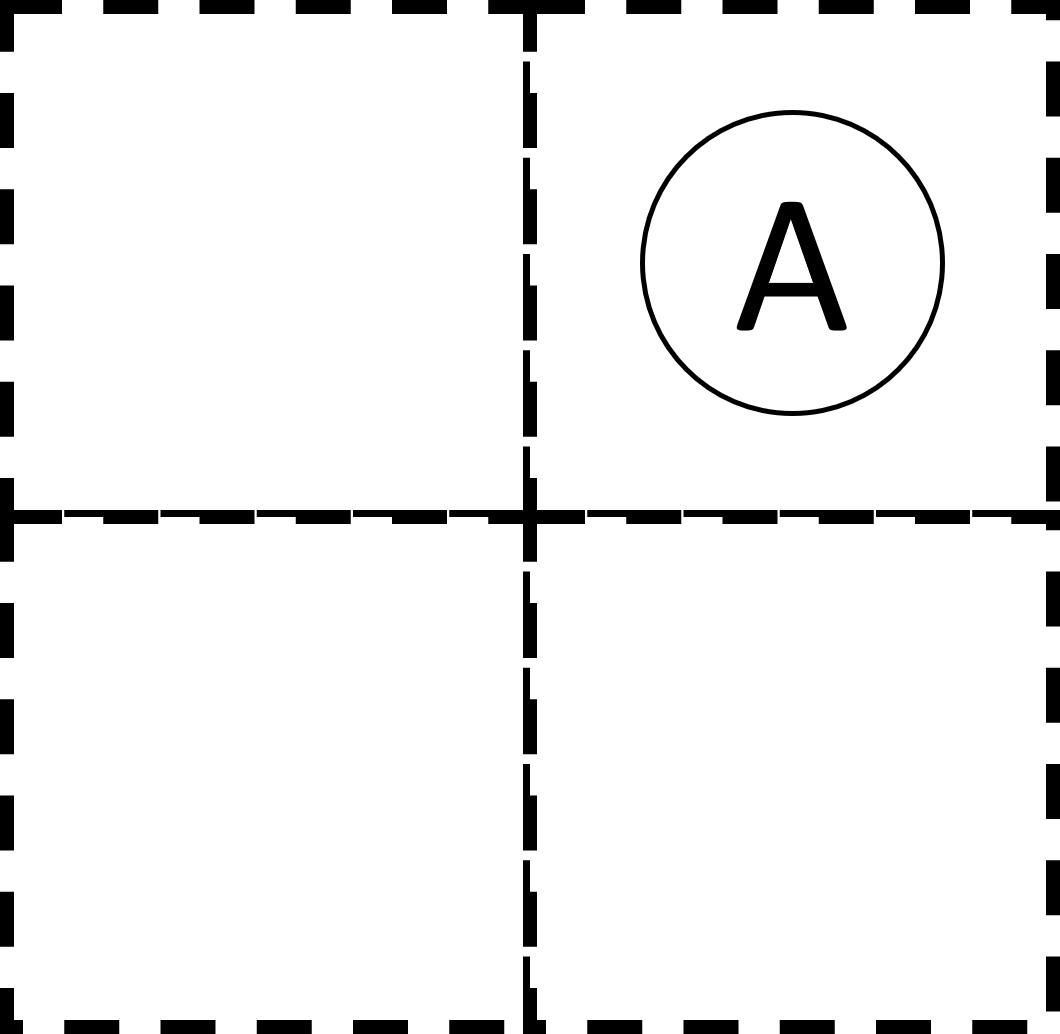
\includegraphics[width=0.5\linewidth]{2MathematicalFramework/Images/2x2_no_walls_world_states/w1.png}
		\caption{$w_{2}$}
		\vspace{0.25cm}
	\end{subfigure}
	\begin{subfigure}[b]{0.45\linewidth}
		\centering
		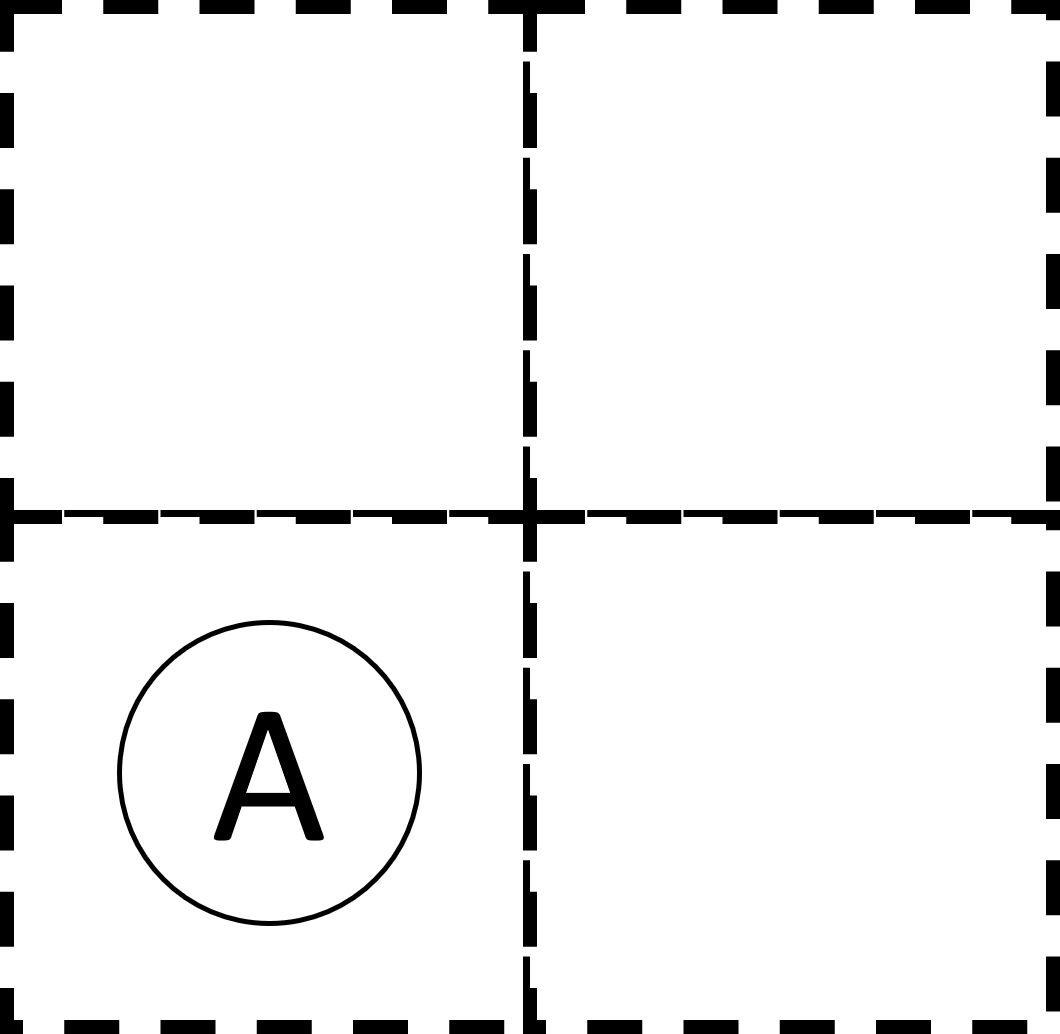
\includegraphics[width=0.5\linewidth]{2MathematicalFramework/Images/2x2_no_walls_world_states/w2.png}
		\caption{$w_{3}$}
	\end{subfigure}
	\begin{subfigure}[b]{0.45\linewidth}
		\centering
		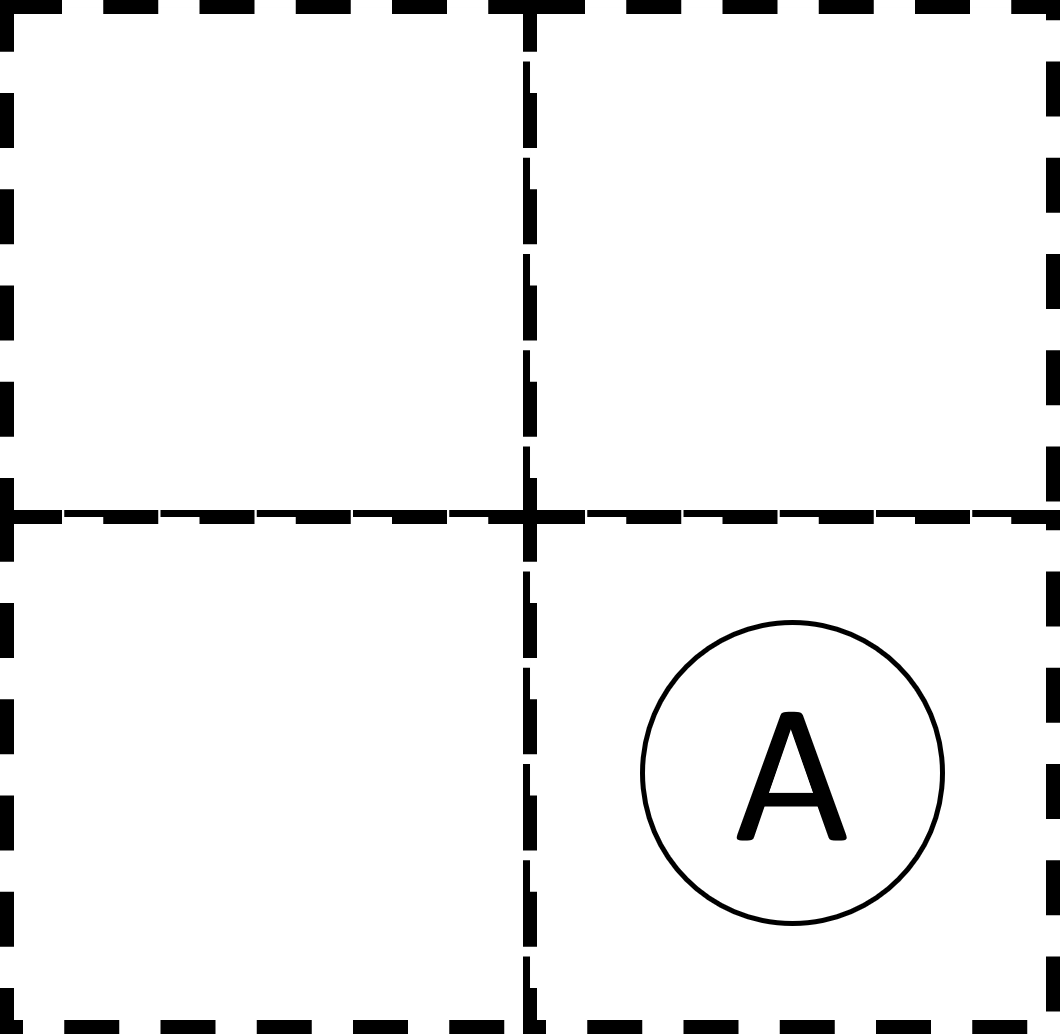
\includegraphics[width=0.5\linewidth]{2MathematicalFramework/Images/2x2_no_walls_world_states/w3.png}
		\caption{$w_{4}$}
	\end{subfigure}
	\caption{
        The world states of a cyclical $2\times 2$ grid world $W_{(2,2)C}$.
        The position of the agent in the world is represented by the position of the circled A.
        }
	\label{fig:2x2-cyclical-grid-world-states}
\end{figure}
\draftnote{purple}{PS: update figure}{
\begin{enumerate}
    \item Update figure using TikZiT.
    \item Make Agent symbol into $\mathscr{A}$.
    \item Include a compass in the figure?
\end{enumerate}
}

%%%%%%%%%%%%%%%%%%%%%%%%%%%%%%%%%%%%%%%%%%%%%%%%%%%%%%%%%%%%%%%%%%%%%%%%%%%%%%%%%%%%%%%%%%%%%%
\subsection{Transformations of $\mathscr{W}_{\alpha}$}

\newthought{There are 24} atomic transformations in $\mathscr{W}_{\alpha}$ (given in \cref{tab:2x2_gridworld_length_1_transformations})\footnote{
    We have chosen these atomic transformations because we know the actions we will give the agent in \cref{sec:Actions of the agent in example}; in reality, the transformations depend on both the structure of the world and the actions of the agent (see proposition \draftnote{blue}{???}{}); in other words, the transformation structure depends on the world-agent pair.
}
and 4 trivial transformations in $D_{\varepsilon}$:
\begin{align}
    & \hat{D} = \hat{D}_{A} = \{ d_{1}, d_{2}, d_{3}, \dots, d_{20} \} \\
    & D_{\varepsilon} = \{1_{w_{1}}, 1_{w_{2}}, 1_{w_{3}}, 1_{w_{4}} \}
    \label{eqn:list_of_D_epsilon}
\end{align}

\begin{table}[H]
    \centering
    \begin{tabular}{c|c c}
        \hline
        Element of $\hat{D}_{A}$ & Source  & Target  \\
        \hline
        $d_{1}$ & $w_{1}$ & $w_{1}$ \\
        $d_{2}$ & $w_{1}$ & $w_{2}$ \\
        $d_{3}$ & $w_{1}$ & $w_{2}$ \\
        $d_{4}$ & $w_{1}$ & $w_{3}$ \\
        $d_{5}$ & $w_{1}$ & $w_{3}$ \\
        $d_{6}$ & $w_{2}$ & $w_{2}$ \\
        $d_{7}$ & $w_{2}$ & $w_{1}$ \\
        $d_{8}$ & $w_{2}$ & $w_{1}$ \\
        $d_{9}$ & $w_{2}$ & $w_{4}$ \\
        $d_{10}$ & $w_{2}$ & $w_{4}$ \\
        $d_{11}$ & $w_{3}$ & $w_{3}$ \\
        $d_{12}$ & $w_{3}$ & $w_{1}$ \\
        $d_{13}$ & $w_{3}$ & $w_{1}$ \\
        $d_{14}$ & $w_{3}$ & $w_{4}$ \\
        $d_{15}$ & $w_{3}$ & $w_{4}$ \\
        $d_{16}$ & $w_{4}$ & $w_{4}$ \\
        $d_{17}$ & $w_{4}$ & $w_{2}$ \\
        $d_{18}$ & $w_{4}$ & $w_{2}$ \\
        $d_{19}$ & $w_{4}$ & $w_{3}$ \\
        $d_{20}$ & $w_{4}$ & $w_{3}$ \\
    \end{tabular}
    \caption{
    The atomic transformations in $\mathscr{W}_{\alpha}$.
    }
    \label{tab:2x2_gridworld_length_1_transformations}
\end{table}

Looking at the world diagram of the atomic multigraph $\hat{\mathscr{W}}_{\alpha}$ of $\mathscr{W}_{\alpha}$ can give us a more intuitive sense of the structure of $\mathscr{W}_{\alpha}$ than looking at the lists of $D_{\varepsilon}$ and $\hat{D}$ in \cref{eqn:list_of_D_epsilon} and \cref{tab:2x2_gridworld_length_1_transformations}:\footnote{
    We have deliberately positioned the vertices of our world diagram of $\hat{\mathscr{W}}_{\alpha}$ to mirror its Euclidean structure (e.g., the line from the $w_{1}$-$w_{2}$ plane is perpendicular to the $w_{1}$-$w_{3}$ plane); however many valid world diagrams of $\hat{\mathscr{W}}_{\alpha}$ do not have this feature.
    For example:
    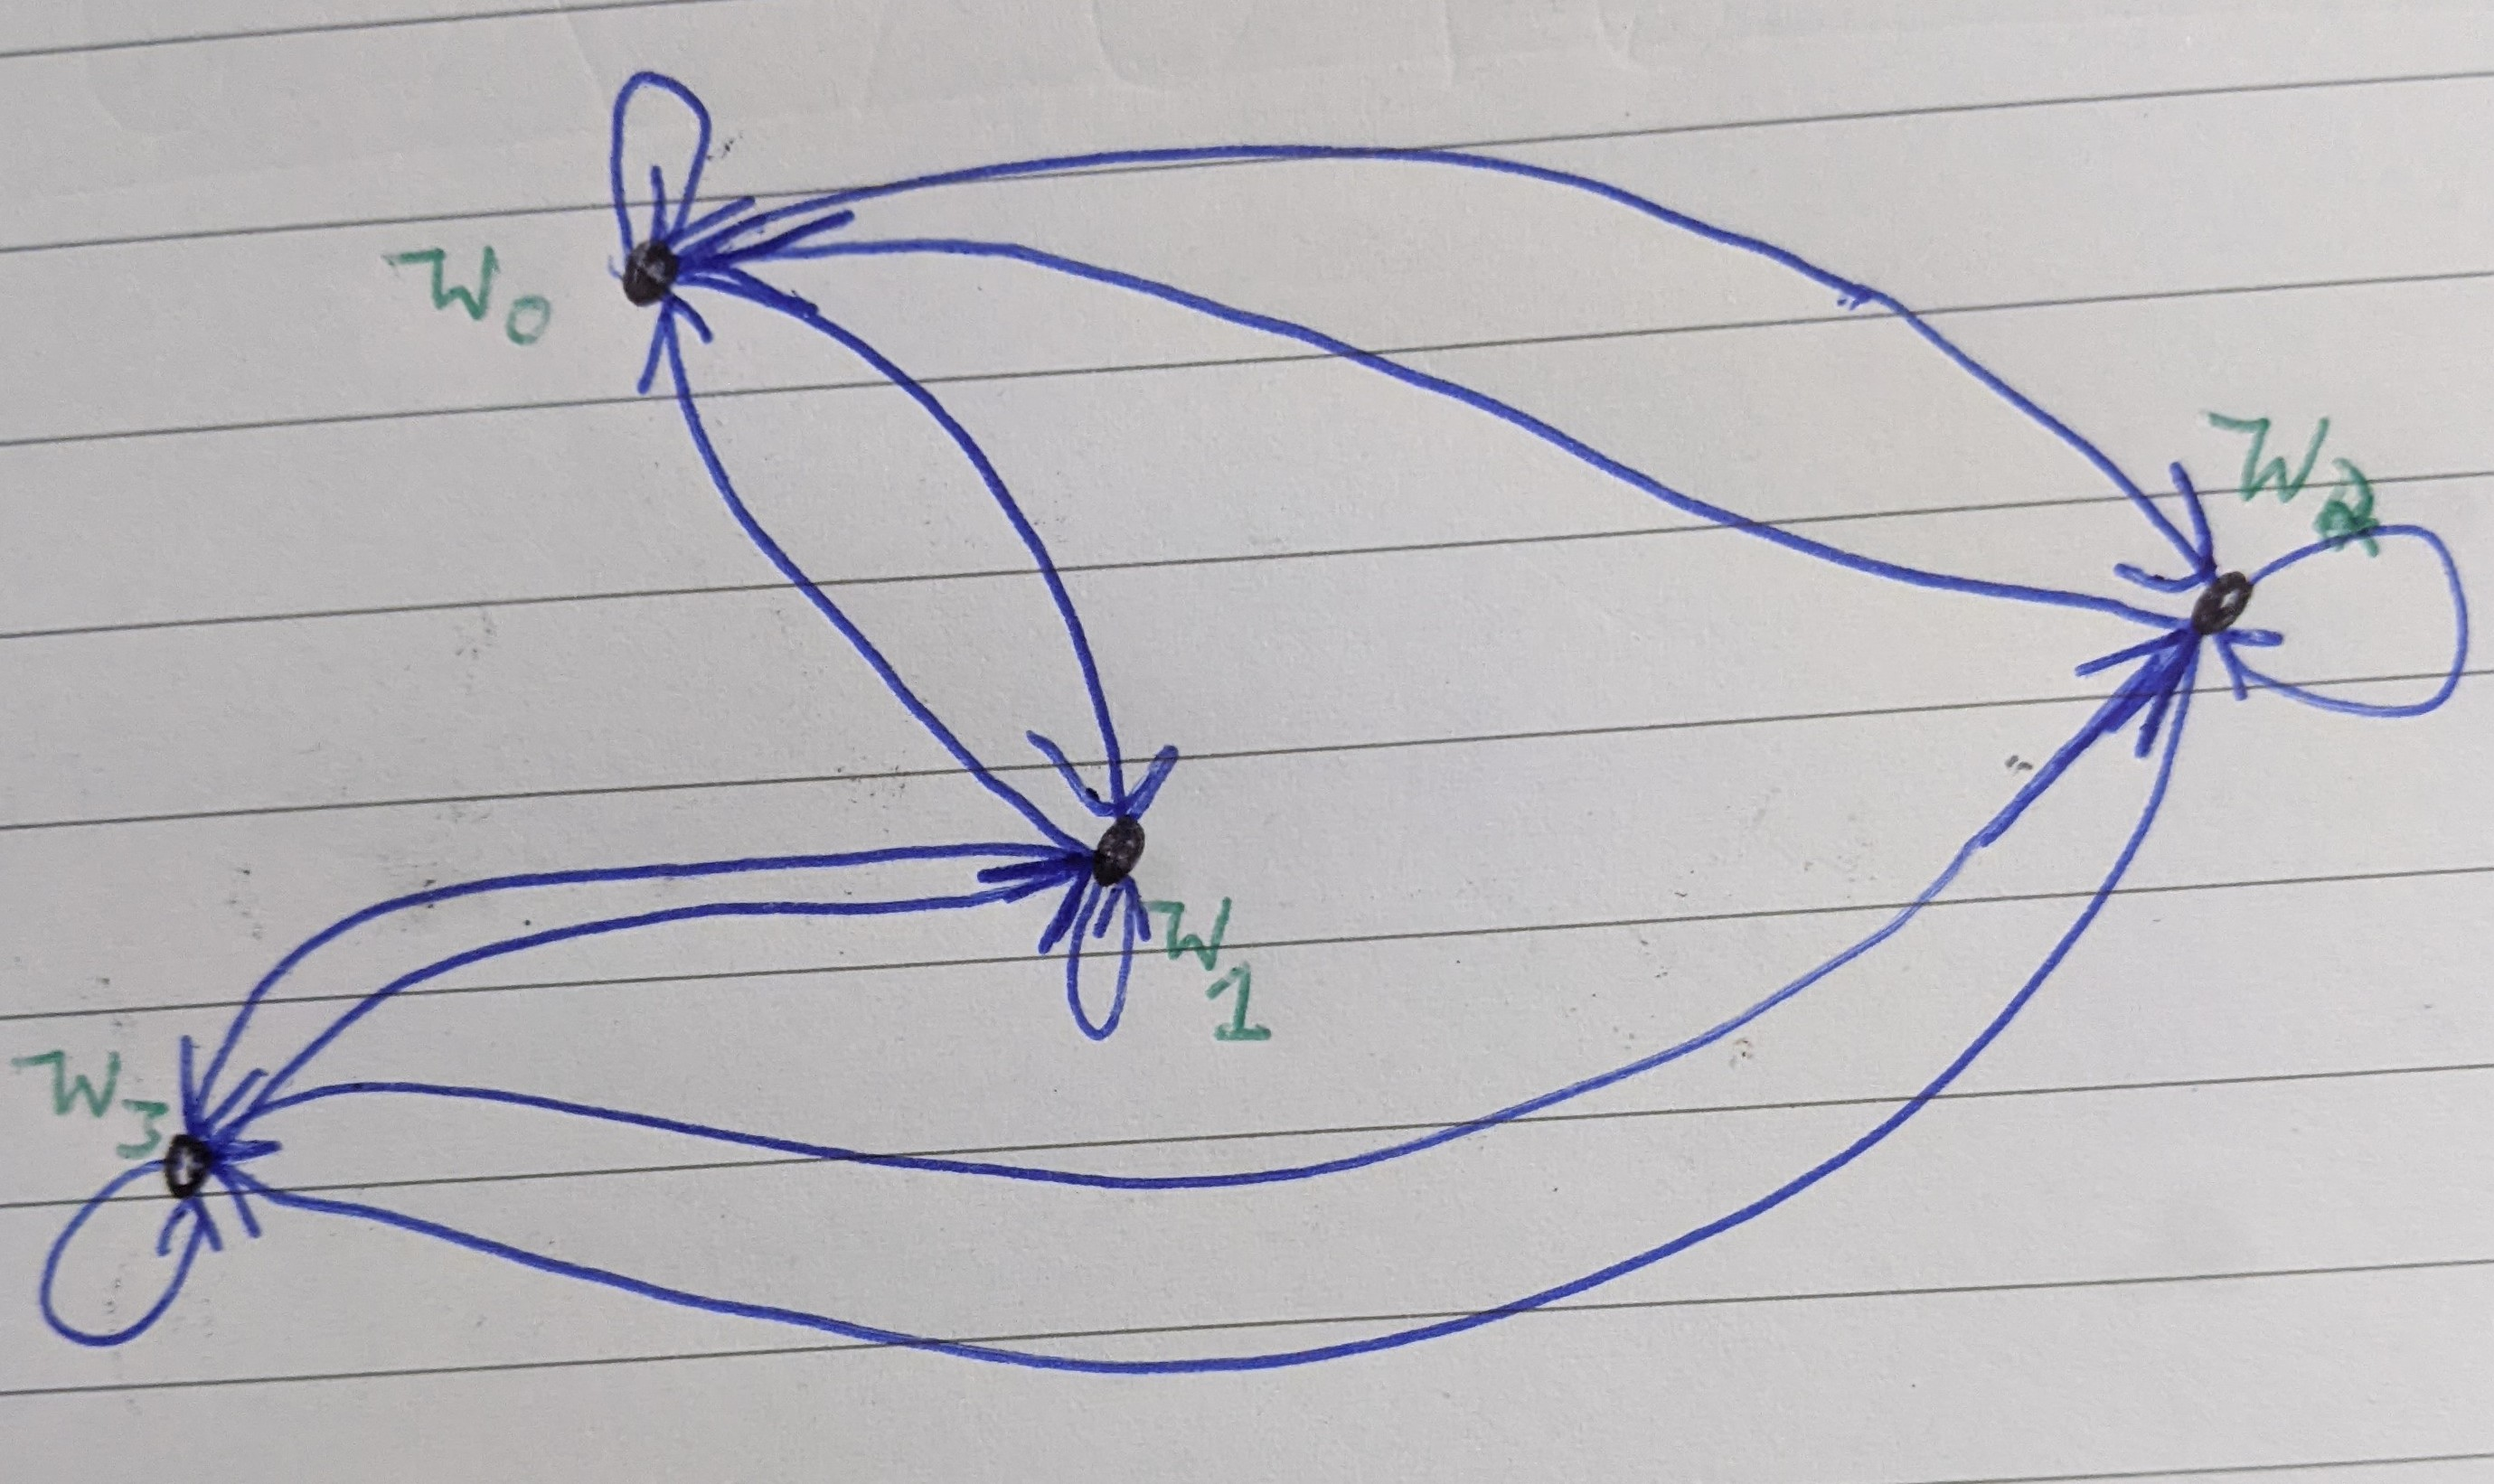
\includegraphics[width=0.5\linewidth]{2MathematicalFramework/Images/2x2_cyclical_min_trans_quirky.jpg}
}

\begin{figure}[H]
    \centering
    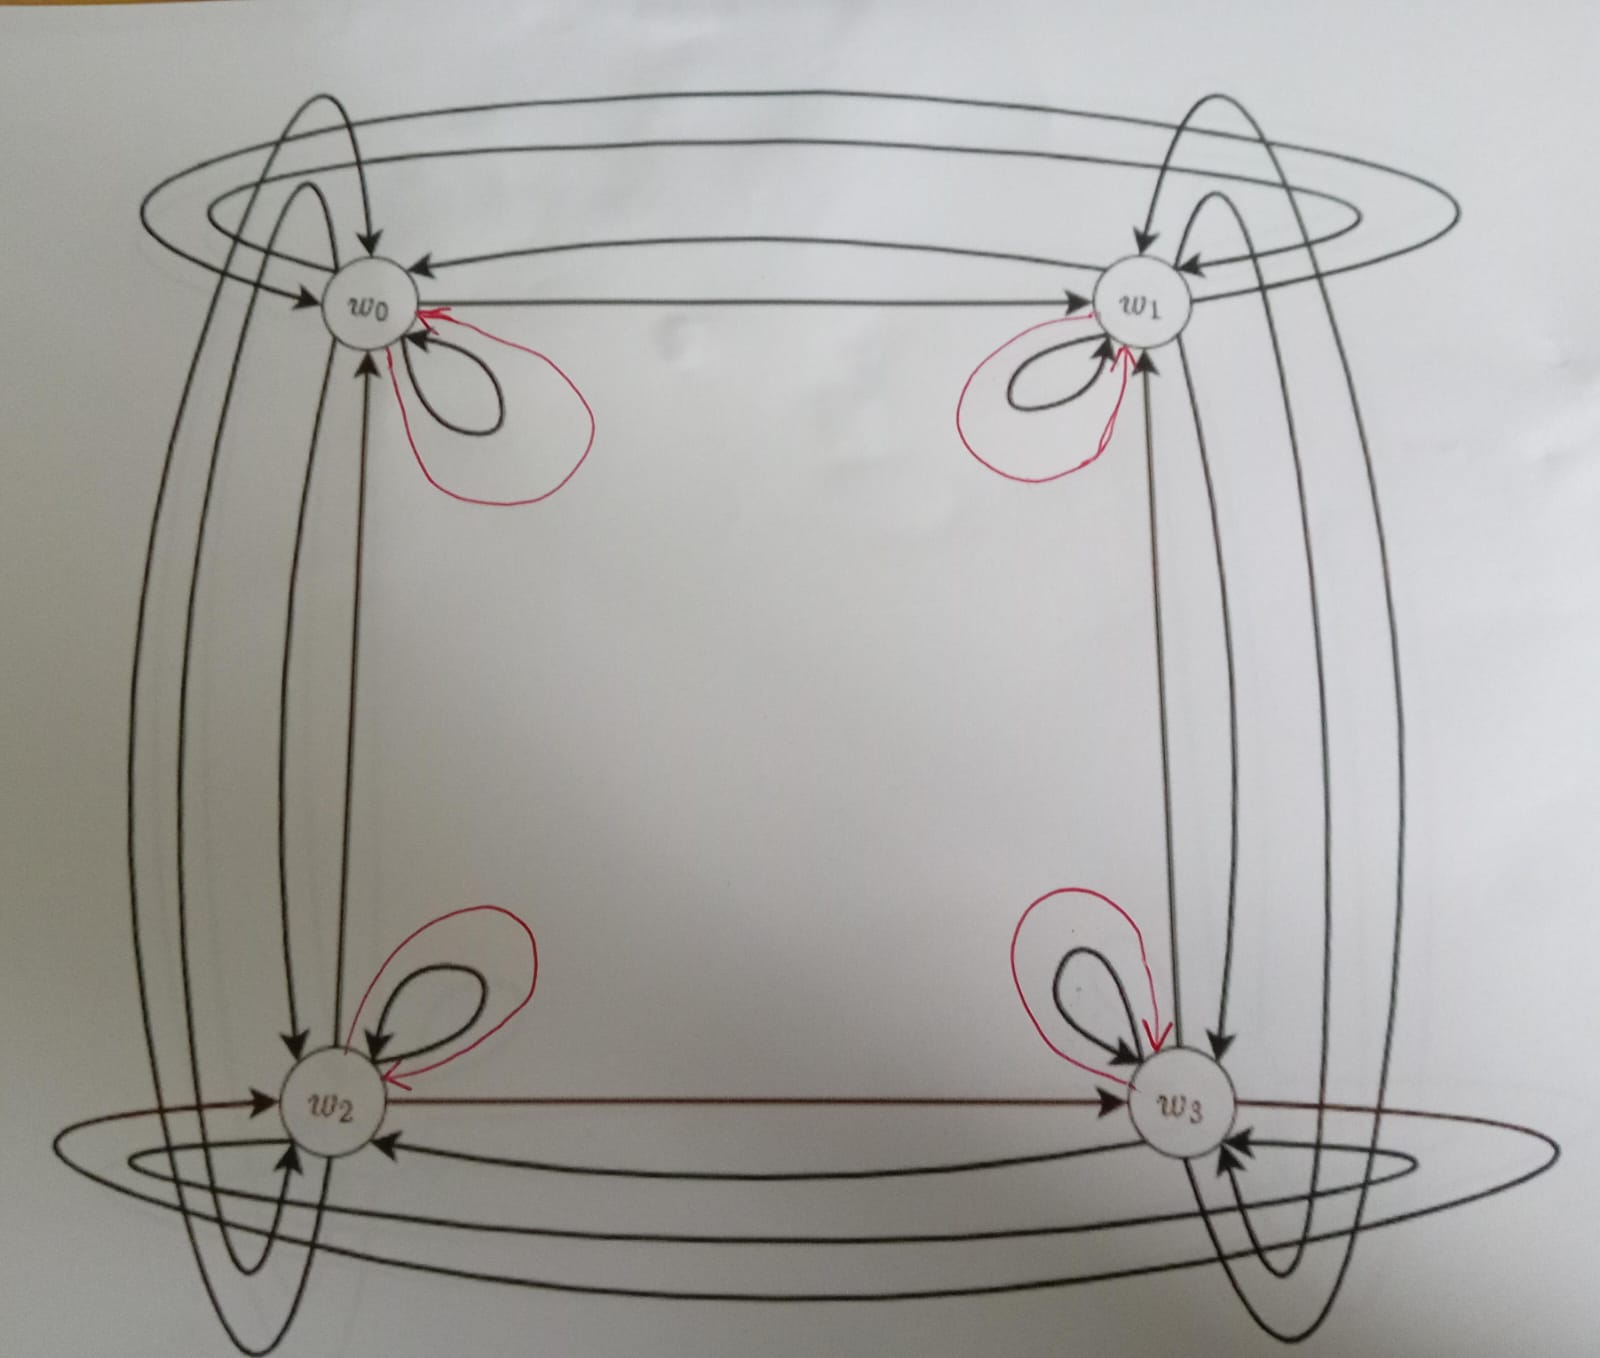
\includegraphics[width=0.5\linewidth]{2MathematicalFramework/Images/2x2_cyclical_minimum_transformations.jpeg}
    \caption{
    A world diagram of $\hat{\mathscr{W}}_{\alpha}$.
    }
    \label{fig:2x2_cyclical_minimum_transformations}
\end{figure}

%%%%%%%%%%%%%%%%%%%%%%%%%%%%%%%%%%%%%%%%%%%%%%%%%%%%%%%%%%%%%%%%%%%%%%%%%%%%%%%%%%%%%%%%%%%%%%
\subsection{Introducing the agent}

\newthought{We consider an} agent $\mathscr{A}$ with ideal sensors, which means there is a one-to-one correspondence between world states visited by the agent and the agent's observations.
Since there are 4 world states, the agent has 4 possible observation states
\begin{equation}
    O = \{ o_{1}, o_{2}, o_{3}, o_{4} \}
\end{equation}
where $b(w_{i}) = o_{i}$.
If the agent's learning process $h$ is perfect, then at the end of the learning process the agent will have four representation state
\begin{equation}
    Z = \{ z_{0}, z_{1}, z_{2}, z_{3} \}
\end{equation}
where $h(o_{i}) = z_{i}$.
Therefore, at the end of the learning process our agent will have a bijective map $f = hb$ where $f(w_{i}) = z_{i}$.

%%%%%%%%%%%%%%%%%%%%%%%%%%%%%%%%%%%%%%%%%%%%%%%%%%%%%%%%%%%%%%%%%%%%%%%%%%%%%%%%%%%%%%%%%%%%%%
\subsection{
Actions of the agent in $\mathscr{W}_{\alpha}$
}\label{sec:Actions of the agent in example}

Our agent $\mathscr{A}$ has the following atomic actions
\begin{equation}
    \hat{A} = \{ a_{1}, a_{U}, a_{D}, a_{R}, a_{L} \}
\end{equation}
as shown in \cref{tab:actions_of_agent_2_by_2_cyclical}.
\begin{table}[H]
    \centering
    \begin{tabular}{l|c}
        \hline
        Action                    & Element of $\hat{A}$ \\
        \hline
        Do nothing (no-op action) & $a_{1}$ \\
        Move up                   & $a_{U}$ \\
        Move down                 & $a_{D}$ \\
        Move right                & $a_{R}$ \\
        Move left                 & $a_{L}$
    \end{tabular}
    \caption{
    Atomic actions of the agent $\mathscr{A}$.
    }
    \label{tab:actions_of_agent_2_by_2_cyclical}
\end{table}

\newthought{Now we have} given the actions in our toy world $\mathscr{W}_{\alpha}$, we can define what we mean by a \emph{cyclical} world.
A world is cyclical if the world returns to its starting state when any action is performed enough times; mathematically, a world $\mathscr{W}$ is cyclical if for any $a \in A$ and $w \in W$, there exists a positive integer $n \in \mathbb{N}^{+}$ such that $a^{n} \ast w = w$\footnote{
    For our example world $\mathscr{W}_{\alpha}$, this means that if the embodied agent $\mathscr{A}$ goes through the top(/bottom/right/left) of side of the world then it will reappear at the bottom(/top/left/right) side; this behaviour is similar to that found in games like Pac-Man \draftnote{blue}{awjdean}{Reference} or Snake \draftnote{blue}{awjdean}{Reference}.
    A more precise example would be that if the embodied agent performs the up action while $\mathscr{W}_{\alpha}$ is in world state $w_{1}$ then $\mathscr{W}_{\alpha}$ will transform into world state $w_{3}$.
}.
In other world, $\mathscr{W}$ forms a Möbius strip with respect to the actions of $\mathscr{A}$.
If the world returns to its starting state when only certain actions are applied enough times, then we say the world is \emph{cyclical with respect to those actions}.

\newthought{Before we can} label the transformations in $D$ with their associated actions, we must identify which transformations should be labelled and how (i.e, we must identify the elements of the sets $\hat{D}_{A}$ and $D_{A}$).
For our example world $\mathscr{W}_{\alpha}$, the procedure outlined in \cref{fig:action_labelling_procedure} in somewhat simplified because all the transformations in $\mathscr{W}_{\alpha}$ are due to the actions of the agent embodied in the world; this means that for our world-agent pair $\mathscr{W}_{\alpha}$-$\mathscr{A}$ we have
\begin{equation}
    \hat{D} = \hat{D}_{A} \\
\end{equation}
and therefore
\begin{align}
    & D = D_{A}, \\
    & \hat{\mathscr{W}} = \hat{\mathscr{W}}_{A}, \\
    \text{and } & \mathscr{W} = \mathscr{W}_{A}.
\end{align}

The atomic action labelling map $\hat{l}$ for $\mathscr{W}_{\alpha}$-$\mathscr{A}$ is given by \cref{tab:2x2_cyclical_labelling_with_min_actions}\footnote{
    Note that the no-op action $1$, where the agent does nothing, does not label the trivial transformations $1_{w}$, which are labelled by the empty action $\varepsilon$.
    This means the no-op action does not necessarily act as an identity element for $(\hat{A}^{*}, \circ, \ast)$.
}, and the atomic action effect operator $\hat{\ast}$ for $\mathscr{W}_{\alpha}$-$\mathscr{A}$ is given by \cref{tab:2x2_gridworld_atomic_action_effect_operator}.

\begin{table}[H]
    \centering
    \begin{tabular}{c|cc||c}
        \hline
        $d \in \hat{D}_{A}$ & $s(d)$  & $t(d)$  & $\hat{l}(d)$ \\
        \hline
        $d_{1}$         & $w_{1}$ & $w_{1}$ & $a_{1}$          \\
        $d_{2}$         & $w_{1}$ & $w_{2}$ & $a_{R}$          \\
        $d_{3}$         & $w_{1}$ & $w_{2}$ & $a_{L}$          \\
        $d_{4}$         & $w_{1}$ & $w_{3}$ & $a_{D}$          \\
        $d_{5}$         & $w_{1}$ & $w_{3}$ & $a_{U}$          \\
        $d_{6}$         & $w_{2}$ & $w_{2}$ & $a_{1}$          \\
        $d_{7}$         & $w_{2}$ & $w_{1}$ & $a_{L}$          \\
        $d_{8}$         & $w_{2}$ & $w_{1}$ & $a_{R}$          \\
        $d_{9}$         & $w_{2}$ & $w_{4}$ & $a_{D}$          \\
        $d_{10}$        & $w_{2}$ & $w_{4}$ & $a_{U}$          \\
        $d_{11}$        & $w_{3}$ & $w_{3}$ & $a_{1}$          \\
        $d_{12}$        & $w_{3}$ & $w_{1}$ & $a_{U}$          \\
        $d_{13}$        & $w_{3}$ & $w_{1}$ & $a_{D}$          \\
        $d_{14}$        & $w_{3}$ & $w_{4}$ & $a_{R}$          \\
        $d_{15}$        & $w_{3}$ & $w_{4}$ & $a_{L}$          \\
        $d_{16}$        & $w_{4}$ & $w_{4}$ & $a_{1}$          \\
        $d_{17}$        & $w_{4}$ & $w_{2}$ & $a_{U}$          \\
        $d_{18}$        & $w_{4}$ & $w_{2}$ & $a_{D}$          \\
        $d_{19}$        & $w_{4}$ & $w_{3}$ & $a_{L}$          \\
        $d_{20}$        & $w_{4}$ & $w_{3}$ & $a_{R}$          \\
        $1_{w_{0}}$     & $w_{1}$ & $w_{1}$ & $\varepsilon$   \\
        $1_{w_{1}}$     & $w_{2}$ & $w_{2}$ & $\varepsilon$   \\
        $1_{w_{2}}$     & $w_{3}$ & $w_{3}$ & $\varepsilon$   \\
        $1_{w_{3}}$     & $w_{4}$ & $w_{4}$ & $\varepsilon$   \\
    \end{tabular}
    \caption{
    The atomic action labelling map $\hat{l}$ for $\mathscr{W}_{\alpha}$-$\mathscr{A}$.
    }
    \label{tab:2x2_cyclical_labelling_with_min_actions}
\end{table}

\begin{table}[H]
    \centering
    \begin{tabular}{c c}
        & Initial world state \\
        Atomic action & \begin{tabular}{c|c c c c}
            $\hat{\ast}$ & $w_{1}$ & $w_{2}$ & $w_{3}$ & $w_{4}$ \\
            \hline
            $a_{1}$ & $w_{1}$ & $w_{2}$ & $w_{3}$ & $w_{4}$ \\
            $a_{U}$ & $w_{3}$ & $w_{4}$ & $w_{1}$ & $w_{2}$ \\
            $a_{D}$ & $w_{3}$ & $w_{4}$ & $w_{1}$ & $w_{2}$ \\
            $a_{L}$ & $w_{2}$ & $w_{1}$ & $w_{4}$ & $w_{3}$ \\
            $a_{R}$ & $w_{2}$ & $w_{1}$ & $w_{4}$ & $w_{3}$ \\
        \end{tabular} \\
    \end{tabular}
    \caption{
    Each entry in this table shows the result of $a_{i} \hat{\ast} w_{j}$ where $a_{i}$ is the row label and $w_{j}$ is the column label.
    \draftnote{purple}{PS}{Fix centering of "Atomic action" and "Initial world state".}
    }
    \label{tab:2x2_gridworld_atomic_action_effect_operator}
\end{table}

The application of the labelling map $\hat{l}$ to the world diagram of $\hat{\mathscr{W}}_{\alpha}$ is shown in \cref{fig:2x2_cyclical_labelling_with_min_actions}.

\begin{figure}[H]
    \centering
    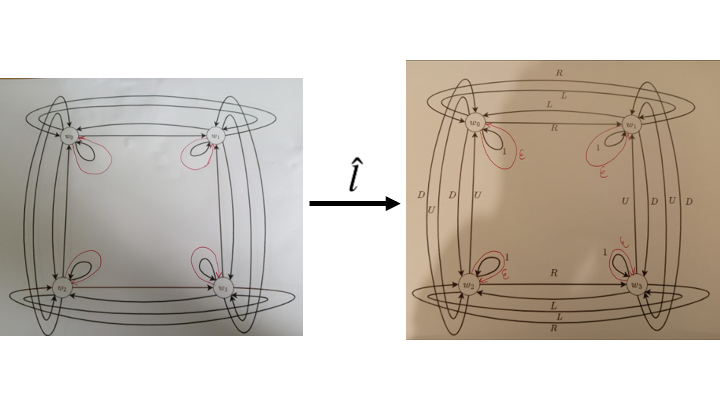
\includegraphics[width=1\linewidth]{2MathematicalFramework/Images/2x2_cyclical_labelling_with_min_actions.png}
    \caption{
    World diagram showing how $\hat{l}$ labels the atomic action transformations and the trivial transformations of $\mathscr{W}_{\alpha}$-$\mathscr{A}$.
    }
    \label{fig:2x2_cyclical_labelling_with_min_actions}
\end{figure}


%%%%%%%%%%%%%%%%%%%%%%%%%%%%%%%%%%%%%%%%%%%%%%%%%%%%%%%%%%%%%%%%%%%%%%%%%%%%%%%%%%%%%%%%%%%%%%
\draftnote{purple}{PS: Consider}{
\begin{enumerate}
    \item (?) Switch $a_{U}$, $a_{D}$, $a_{R}$, $a_{L}$ to $a_{N}$, $a_{S}$, $a_{E}$, $a_{W}$ --> makes sense when giving agent ability to rotate.
    \item Show parts of: $\hat{A}^{*}$, $D$.
    \item Diagram (l-map-for-transformations-from-and-to-w0) - demonstrates how the map $\hat{l}$ maps transformations in $\hat{D}_{A}$ to the elements in $\hat{A}$.
\end{enumerate}
}
